\documentclass{tcc}

% MACROS E DEFINIÇÕES
\newcommand{\Red}[1]{{\color{red}#1}} 
\newcommand{\Mag}[1]{{\color{magenta}#1}} 

\numberwithin{equation}{section}
\definecolor{lightgray}{rgb}{0.95,0.95,0.95}

%% --- LISTINGS
\lstset{language=python,
	%basicstyle=\ttfamily,
	backgroundcolor=\color{lightgray},
	numbers=left,
	numberstyle=\footnotesize,
	frame=trbl,
	frameround=tttt,
	showstringspaces=false,
	tabsize=3,
}
%\lstset{frame=lines}
%\lstset{label={lst:code_direct}}
%\lstset{basicstyle=\footnotesize}

\begin{document}

%% --- SETUP 
%Dados do TCC%
\author{Silas Aguiar Melo}
\title{Análise por Elementos Finitos da Eficiência de Varrido de Colchões Lavadores em Anulares Afetados por Excentricidade e Erosões}
\newcommand{\subtitulo}{}
\newcommand{\nomedocurso}{Matemática Computacional}
\newcommand{\titulobar}{titulo}
\newcommand{\orientador}{Gustavo Charles Peixoto de Oliveira}
\newcommand{\profa}{Gustavo Charles Peixoto de Oliveira}
\newcommand{\profb}{Moisés Dantas dos Santos}
\newcommand{\profc}{Gustavo Rabello dos Anjos}
\newcommand{\profd}{Bruno Leonardo de Sena Costa}
\newcommand{\insta}{Universidade Federal da Paraíba}
\newcommand{\instb}{Universidade Federal da Paraíba}
\newcommand{\instc}{Universidade Federal do Rio de Janeiro}
\newcommand{\instd}{Universidade Federal do Rio Grande do Norte}
\newcommand{\coordenador}{Roberto Quirino do Nascimento}
\newcommand{\departamento}{Curso}

%% --- ELEMENTOS PRÉ-TEXTUAIS 

%% ------- CAPA
\pagestyle{empty} %retira numeração da página
% TITULO
\begin{center}
\LARGE{\bf \thetitle}\\
%\Large{\bf \subtitulo}\\
\end{center}
\vspace{1em}
% AUTOR
\begin{center}
\theauthor
\end{center}
\vfill
% LOGO CI
\begin{figure}[H]
\centering
	
\includegraphics[width=3cm]{img/logo-ci.png}
\end{figure}
\begin{center}
CENTRO DE INFORMÁTICA \\
UNIVERSIDADE FEDERAL DA PARAÍBA
\end{center}
\vfill
\begin{center}
João Pessoa, \the\year
\end{center}
% ESTA PÁGINA EM BRANCO É NECESSÁRIA? SE SIM, DESCOMENTE.
%\afterpage{\blankpage \addtocounter{page}{1}} %addtocounter incrementa numero da pagina ja que blankpage nao entra no contador%
%% ------- ROSTO
\newpage
\begin{center}
\theauthor
\end{center}
\vfill
\begin{center}
\LARGE{\thetitle}\\
\end{center}
\vfill
\begin{flushright}
\parbox{8.85cm}{
\singlespacing{TCC apresentado ao curso de \nomedocurso do Centro de Informática, da Universidade Federal da Paraíba, como requisito para a obtenção do grau de Bacharel em \nomedocurso.}}
\\
\vspace{0.2in}
Orientador: \orientador
\end{flushright}
\vfill
\begin{center}
\MONTH de \the\year
\end{center}
%% ------- FOLHA CATALOGRÁFICA
\newpage
\phantom{}
\vfill
\begin{flushright}
\fbox{\parbox[t][15em][c]{0.90\linewidth}{
\vspace{0.5in}

\hspace{2em}
Ficha catalográfica: elaborada pela biblioteca do CI. 
\vspace{0.15in}

\hspace{2em}
Será impressa no verso da folha de rosto e não deverá ser contada. 

\hspace{2em}
Se não houver biblioteca, deixar em branco.
}}
\end{flushright}
%% ------- FOLHA DE APROVAÇÃO
\newpage
\begin{figure}[H]
\centering

\includegraphics[width=2cm]{img/logo-ci.png}
\end{figure}

\begin{center}
CENTRO DE INFORMÁTICA \\
UNIVERSIDADE FEDERAL DA PARAÍBA
\end{center}

\vspace{1cm}

\noindent Trabalho de Conclusão do Curso de \nomedocurso intitulado \textit{\bf \em \thetitle}, de autoria de \theauthor, aprovado por Banca Examinadora constituída pelos seguintes membros: \\

\vspace{0.5in}

\hrule
\noindent Prof. Dr. \profa\\
\insta\\

\vspace{0.2in}

\hrule
\noindent Prof. Dr. \profb\\
\instb\\

\vspace{0.2in}

\hrule
\noindent Prof. Dr. \profc\\
\instc\\

\vspace{0.2in}

\hrule
\noindent Dr. \profd\\
\instd\\

\vspace{2cm}
\vfill

\hrule
\noindent Coordenador(a) do \departamento\\
Prof. Dr. \coordenador\\
%CI/UFPB\\

\vfill

\begin{center}
João Pessoa, \today
\end{center}

%% PRECISA DE ENDEREÇO AQUI??
%\vspace{0.05in}
%\begin{center}
%\footnotesize{Centro de Informática, Universidade Federal da Paraíba\\
%Rua dos Escoteiros, Mangabeira VII, João Pessoa, Paraíba, Brasil CEP: 58058-600\\
%Fone: +55 (83) 3216 7093 / Fax: +55 (83) 3216 7117}
%\end{center}
%% PRECISA DESSA?
%\afterpage{\blankpage \addtocounter{page}{1}}
%página em branco%
\section*{\centering{DEDICATÓRIA}} 
\phantom{}\\
\null
\vfill
\begin{center}
\noindent Ao Senhor.
\end{center}

%\newpage

\section*{\centering{AGRADECIMENTOS}}

Ao Senhor Jesus. Não há como iniciar meus agradecimentos de outra forma, todo o crédito vai para Ele, pois sem Ele, nada do que foi feito se fez. Ele me deu a vida, o ânimo e a saúde para que eu pudesse realizar este sonho. Ele é o responsável pela oportunidade que tive de entrar em uma Universidade Federal em um Estado diferente daquele que nasci e morei toda a minha vida. Por Ele ser minha fortaleza, consegui concluir o curso.
Agradeço aos meus pais que me colocaram no mundo, me educaram e cuidaram de mim. Apesar da simplicidade em que vivíamos, sempre deram o melhor de si para que eu tivesse um futuro profissional realizado. À minha mãe que sempre acreditou em mim e que nunca deixou de me ajudar em oração. Ao meu padastro que lutou por mim, sem ele não teria nem chegado em João Pessoa, não há palavras para expressar minha gratidão. Aos meus irmãos que mesmo sem saberem, também me deram forças para continuar. À minha namorada Mayara que também é minha amiga querida desde sempre, me deu ânimo, forças e alegria para perseverar.
Ao professor Gustavo, com sua imensa paciência com que me ensinou e orientou, não desistiu de mim.
Ao meu amigo e irmão em Cristo Jesus, Rinaldo, que sempre me incentivou e alimentou o desejo de seguir em frente mesmo em meio às tribulações, me encorajou e me inspirou em muitas coisas.
À dona Áurea, diretora da escola quando estudei o ensino fundamental, que, da maneira como cuidava da escola, me fez um bom aluno.
Ao Prof. Edvaldo que me inspirou a seguir a área de exatas, sempre me incentivou e acreditou em mim, e falando sobre mim à outros alunos, me motivava a terminar o curso e ser sempre um bom aluno para não o decepcionar. À minha amiga Ana Paula que me indicou a melhor escola de Ensino Médio. À escola Jarina Maia por todo preparo para me levar até à graduação. Aos meus caros professores do ensino médio Ione, Cristina Portela, Lelo, Almir, Cristina Moura, Eli, etc.
Ao ChiAlpha, à cru, aos meus amigos ...
\newpage

\section*{\centering{RESUMO}} 

\noindent
A cimentação primária de poços é uma fase crucial das atividades de \textit{upstream} na indústria de petróleo e gás para proteger o revestimento metálico instalado no poço, impedir a migração de fluidos por meio de fraturas e impedir efeitos adversos no espaço anular. Em particular, colchões lavadores são aplicados com a finalidade de remover impurezas remanescentes após a perfuração e  facilitar a aderência do cimento à parede porosa. Neste trabalho, analisamos o comportamento hidrodinâmico de um colchão lavador com propriedades físicas equivalentes a de uma emulsão à base de óleo vegetal no espaço anular existente entre o revestimento (\textit{casing}) e a formação rochosa. O escoamento é simulado de maneira simplificada usando a hipótese de fluido Newtoniano, modelado pelas equações de Navier-Stokes para o caso incompressível. Simulações numéricas são executadas via método de elementos finitos a partir da biblioteca FEniCs para configurações bidimensionais representativas de poços submetidos a excentricidades (taxas de \textit{standoff} menores do que 100\%) e erosões. Por fim, comparamos os efeitos de \textit{standoff} e de erosões com modelos homólogos não erodidos e calculamos a eficiência de varrido para caso particular. Os resultados mostram que o perfil de velocidade é alterado quando consideramos malhas cujos contornos assemelham-se a paredes erodidas.

\vspace{1cm}

\noindent{\bf Palavras-chave:}
petróleo e gás,
cimentação primária, 
limpeza de poços, 
dinâmica dos fluidos computacional.
\newpage
\section*{\centering{ABSTRACT}} 

\noindent 
Primary well cementing is a crucial stage of upstream activities in the oil and gas industry to protect the metallic casing inside the well, prevent fluid migration through fractures and avoid adverse effects on the annular space. In particular, flusher fluids are applied to clean post-drilling impurities and facilitate cement's adhesion to the porous wall. In this report, we analyzed the hydrodynamic behavior of a flusher with physical properties equivalent to a vegetable oil-based emulsion moving through the annular space between the casing and the rock formation wall. The incompressible fluid flow was simulated under a Newtonian hypothesis and modeled by the Navier-Stokes equations. Numerical simulations were performed via finite element method from the FEniCs library for two-dimensional configurations representing wells subjected to standoff rates less than 100\% and erosion. Finally, we compared the effects of eccentricity and erosions against homologous non-eroded models and calculated the sweep efficiency for each case. Our findings show that the velocity profile is changed when one consider meshes whose boundaries mimic eroded walls.

\vspace{1cm}

\noindent{\bf Keywords:} 
oil and gas,
primary cementing, 
well cleaning, 
computational fluid dynamics.

\newpage
\renewcommand{\listfigurename}{\centering LISTA DE FIGURAS}
\listoffigures
\newpage
\renewcommand{\listtablename}{\centering LISTA DE TABELAS}
\listoftables
%\newpage
\section*{\centering{LISTA DE ABREVIATURAS}} 


%% SUMÁRIO
\newpage
\pagestyle{plain} %mostra numeração da página%
\tableofcontents
\newpage

%% --- ELEMENTOS TEXTUAIS 

\section{INTRODUÇÃO}

O primeiro poço de petróleo foi perfurado na Pensilvânia, Estados Unidos, em meados do século XIX. Esse poço tinha apenas 23 metros de profundidade quando começou seu ciclo produtivo. Naquela época, o petróleo, até então utilizado como combustível para lamparinas a óleo, gradativamente passou a ser destilado para produzir combustíveis, como o querosene. A descoberta de novas jazidas faria surgir cidades em pleno deserto americano, caracterizando o início da febre do ``ouro negro''. Dali em diante, a tecnologia envolvida na perfuração de poços de petróleo evoluiu consideravelmente e, com o advento da computação, houve grandes melhorias nos processos de extração \cite{Max}.

A história do petróleo no Brasil começa com Eugênio Ferreira de Camargo, quem, em 1892, tentou encontrar petróleo na cidade paulista de Bofete após perfurar um poço de 488 metros. Todavia, achou-se apenas água. Essa foi a primeira tentativa para encontrar petróleo no Brasil. Entretanto, apenas em 1939 descobriu-se a primeira jazida de petróleo na cidade de Salvador, Bahia \cite{Danilo}.

A demanda por petróleo ainda é elevada, visto que é matéria-prima para muitos produtos derivados, tais como plástico, asfalto e gasolina. Com o avanço tecnológico dos processos de recuperação, a indústria de petróleo e gás passou a explorar o recurso em lugares cada vez mais profundos, às vezes ultrapassando os 5000 metros, a exemplo do petróleo retirado do Pré-Sal brasileiro \cite{Petrobras}. Entretanto, essa enorme profundidade leva a desafios operacionais no âmbito da perfuração, completação e estabilidade dos poços.

Durante a atividade de perfuração, injeta-se um fluido por dentro da coluna de perfuração, que avança desde a superfície até à broca. Na broca há um orifício por onde ele é expelido e segue o seu caminho de retorno à superfície passando pelo espaço anular existente entre a coluna de perfuração e a parede do poço. Durante o movimento de retorno, o fluido transporta cascalhos ou fragmentos de rocha que são gerados pela perfuração da formação. Esse fluido é chamado de \textit{fluido de perfuração} \cite{Escudier}.

No processo de perfuração, introduz-se um revestimento metálico com o intuito de proteger e isolar a formação rochosa \cite{KOEHLER}. Em seguida, o espaço anular compreendido entre o revestimento e a formação necessita de preenchimento. Esse preenchimento é realizado por meio do processo de cimentação \cite{SANTOS}. A cimentação é uma das fases mais importantes na  construção de poços de petróleo, a qual tem por função proteger o revestimento metálico instalado no poço e assim impedir o movimento de fluidos através do espaço anular \cite{Bourgoyne}. 

O fluido de perfuração e a pasta de cimento são na maioria das vezes incompatíveis. Por isso, é necessário remover o fluido de perfuração para que a pasta de cimento tenha aderência à formação rochosa. Para tanto, são injetados fluidos intermediários antes da injeção do cimento que são chamados de ``colchões'' (\textit{flushers}), a saber, o ``colchão lavador'' e o ``colchão espaçador''. Esses fluidos têm como função remover completamente o fluido de perfuração da parede do poço \cite{ARANHA}.

Há inúmeros desafios na extração do petróleo. Quanto mais profundo o poço, mais problemas surgem. Um desses problemas é a ocorrência de deslocamento por excentricidade, fenômeno usualmente chamado de \textit{standoff}. O \textit{standoff} ocorre quando o revestimento é inserido no poço e não se conforma perfeitamente centralizado até o fundo do poço, causando má eficiência no processo de limpeza. Consequentemente, a aderência do cimento à formação torna-se comprometida, provocando potenciais problemas de infiltração de fluidos indesejáveis para o interior do poço, além de problemas mecânicos e estruturais, tais como fraturas que podem induzir a demolição do poço \cite{Erik}. 

O presente trabalho analisa o comportamento hidrodinâmico de um colchão lavador com propriedades físicas equivalentes às de uma emulsão a base de óleo vegetal no espaço anular existente entre o revestimento (\textit{casing}) e a formação rochosa. Realizamos simulações de escoamento de maneira simplificada usando a hipótese de fluido newtoniano, modelado pelas equações de Navier-Stokes para o caso incompressível. Os experimentos numéricos são executados via método de elementos finitos a partir da biblioteca FEniCS para configurações bidimensionais representativas de poços submetidos a excentricidades (taxas de \textit{standoff} menores do que 100\%) e erosões. Por fim, os efeitos de \textit{standoff} e de erosões foram comparados com modelos homólogos não erodidos e foi calculada a eficiência de varrido para o caso particular.

 % Revisado
\section{REVISÃO BIBLIOGRÁFICA}

\subsection{Mecânica dos Fluidos Aplicada à Engenharia de Poços de Petróleo}
	
Fluidos são substâncias capazes de escoar que se deformam com facilidade. Gases, líquidos e inclusive o plasma são classificados como fluidos. A mecânica dos fluidos está presente em uma vasta gama de situações: sistema respiratório e circulatório, esportes náuticos, bombas hidráulicas, ventiladores, turbinas, aviões, navios, rios, moinhos de vento, mísseis supersônicos, icebergs, motores, filtros, jatos e sprinklers. Quase tudo no mundo é um fluido ou se move dentro ou perto de um fluido \cite{White}. 
		
Os fluidos podem ser newtonianos ou não newtonianos. Fluido newtoniano é aquele que a viscosidade, ou atrito interno, é constante para diferentes taxas de cisalhamento. Nos fluidos newtonianos, a tensão é diretamente proporcional à taxa de deformação. Apesar de não existir um fluido perfeitamente newtoniano, fluidos considerados homogêneos, como a água e o ar, costumam ser estudados como newtonianos para muitas finalidades práticas \cite{Pordeus}.
		
		
Fluido não-newtoniano é aquele cuja viscosidade varia proporcionalmente à energia cinética que se imprime a esse mesmo fluido, respondendo de forma quase instantânea. Para exemplo temos a mistura do amido de milho com água que, dependendo da pressão que recebe, pode ser um sólido ou um líquido, apresentando característica viscosa. Com pressão suficiente, torna-se um sólido e com menor pressão volta ao estado líquido \cite{Pordeus}.
		
		
Outra característica de um fluido diz respeito à sua compressibilidade. Um fluido \emph{compressível} é aquele que possui a habilidade de ser comprimido em um recipiente quando seu volume diminui por ação de uma força aplicada. A massa específica do fluido muda em relação ao grau de compressão sofrido . Já um fluido \textit{incompressível} é aquele cuja massa específica permanece relativamente constante, ou seja, que resiste à redução de seu volume quando submetido a uma força compressiva \cite{Pordeus}.
		
\subsubsection{Colchões}

Para que haja remoção eficiente do fluido de perfuração na parede da formação no interior dos poços de petróleo, são injetados fluidos denominados colchões lavadores e colchões espaçadores antes da pasta de cimento, como dito anteriormente. Estes colchões têm distintas finalidades durante o processo de limpeza do poço.
			
Colchão lavador é um fluido com baixa viscosidade e baixa massa específica compatível com o fluido de perfuração. Por meio de ações químicas e mecânicas, ele dilui e remove o reboco (camada de baixa permeabilidade formado pelos fluidos de perfuração nas paredes do poço).

Colchão espaçador é, geralmente, um fluido com viscosidade e massa específica altas que atua apenas de forma mecânica para a remoção do reboco. Semelhantemente aos colchões lavadores, também são injetados antes da pasta de cimento com o intuito de evitar o contato dela com o fluido de perfuração. Eles ajudam a preservar eventuais problemas de cimentação, a exemplo da formação de canais de fluido no interior do cimento que prejudicam o isolamento hidráulico \cite{Campos}.
			
A Fig. \ref{fig:remocao_fluido} ilustra o funcionamento dos colchões na engenharia de poços. Podemos observar que o colchão lavador (cor azul clara), depois de injetado pelo interior do revestimento, retorna à superfície pelo espaço anular empurrando o fluido de perfuração responsável pelo carreamento de detritos (cor marrom). Em seguida, o colchão espaçador (cor verde), remove o restante dos fluidos anteriormente injetados para que a pasta de cimento (cor cinza) se adira às paredes da formação adequadamente \cite{Campos}.
\begin{figure}[H]
    \centering
    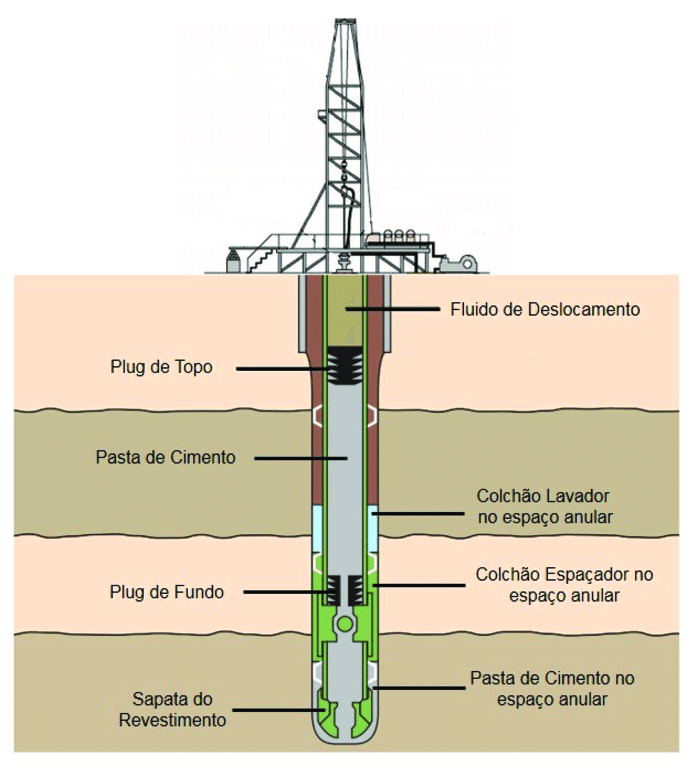
\includegraphics[scale=0.35]{img/remocao_fluido.png}
    \caption
    [Remoção de fluido de perfuração por ação de colchões (lavador e espaçador) durante a cimentação primária de um poço de petróleo.]
    {Remoção de fluido de perfuração por ação de colchões (lavador e espaçador) durante a cimentação primária de um poço de petróleo. Fonte: \cite{Curbelo}.}
    \label{fig:remocao_fluido}
\end{figure}
		
	
\subsubsection{Excentricidade do Tubo de Revestimento}

Quando o eixo do tubo de revestimento (\textit{casing}) coincide com o eixo do poço perfurado, diz-se que o arranjo está sob uma configuração anular concêntrica. Neste caso, os fluidos deslocam-se no espaço anular de maneira relativamente simétrica, proporcionando aos processos de limpeza e cimentação certo grau de uniformidade na parede do poço. Entretanto, quando o tubo de revestimento está deslocado do centro, a configuração do anular torna-se excêntrica, os colchões tendem a fluir de maneira não uniforme. A presença de excentricidade (\textit{standoff}) no tubo de revestimento é um fator que influencia fortemente o deslocamento de fluidos durante os processos de perfuração e completação de poços de petróleo.

O comprometimento da eficiência de varredura pode ocorrer com qualquer fluido injetado, inclusive com a pasta de cimento. Em geral, para que não haja pontos da formação com lacunas de cimentação, centralizadores são instalados no tubo para manter o espaço anular o mais uniforme possível. 
A excentricidade entre poço e revestimento é medida, em geral, por um parâmetro popularmente conhecido como \textit{standoff}. A taxa de standoff pode ser representada por um percentual que varia entre 0\% (revestimento em contato com a parede) e 100\% (revestimento afastado ao máximo da parede). Entretanto, os limites inferior e máximo são praticamente inatingíveis, permanecendo a taxa em valores intermediários. 
Obter valores genuinamente altos de \textit{standoff} é uma tarefa extremamente difícil para a engenharia de poços. Além disso, o próprio revestimento pode dobrar ou ceder em alguns pontos no interstício entre um centralizador e outro, resultando em um \textit{standoff} notadamente menor (\textit{sag point}). Por isso, durante o trabalho de limpeza, o colchão lavador encontrará maior resistência para deslocar o fluido de perfuração na porção anular que estiver espremida, deixando para trás resquícios de detritos não carreados. Um exemplo desse problema é mostrado na Fig. \ref{fig:Standoff1}, relativo a um incidente ocorrido com o poço de Macondo, no Golfo do México, em 2011 
\cite{Macondo,Hanieh}.
\begin{figure}[H]
	\centering
	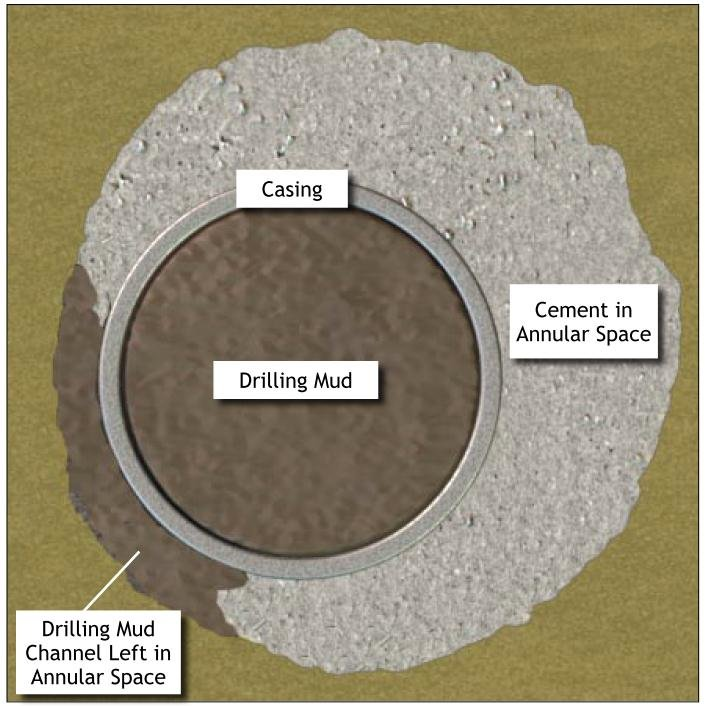
\includegraphics[scale=0.7]{img/Standoff1.png}
	\caption[Seção transversal de um revestimento excêntrico.]{Seção transversal de um revestimento excêntrico.}
	\label{fig:Standoff1}
\end{figure}
A Fig. \ref{fig:Standoff2} mostra um caso de \textit{standoff} menor entre dois centralizadores \cite{VADIM}.
\begin{figure}[H]
	\centering
	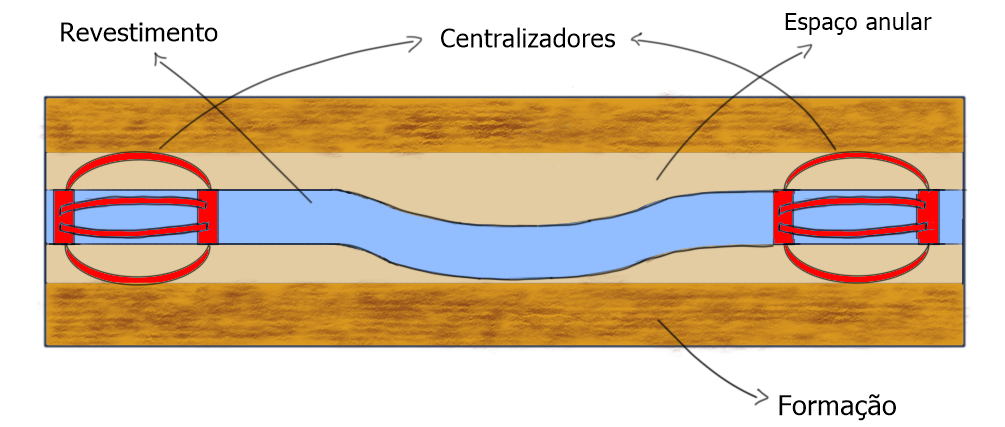
\includegraphics[width=0.7\linewidth]{img/centralizadores_standoff.png}
	\caption[\textit{Standoff} menor do que 100\% entre dois centralizadores.]{\textit{Standoff} menor do que 100\% entre dois centralizadores. Fonte: autor.}
	\label{fig:Standoff2}
\end{figure}

Considerando a seção transversal de um anel excêntrico, como se vê na Fig. \ref{fig:secao_transversal_equivalente_livro}, a taxa de \textit{standoff} pode ser calculada como \cite{Erik}: 
\begin{equation}
    \varsigma = (1 - \alpha) 100\%, \quad \text{com} \quad \alpha = \frac{e}{r_o - r_i},
\end{equation}
onde $e$ é a distância entre o centro do poço e o centro do tubo de revestimento, $r_o$ é o raio do poço e $r_i$ é o raio do tubo de revestimento. O cálculo do \textit{standoff} usa um ponto de referência na parede do poço para definir o afastamento, especificamente na interseção inferior que se acha entre a circunferência do poço aberto e a linha de simetria que passa pelo ângulo desdobrado de $\pi$ radianos (Fig. \ref{fig:secao_transversal_equivalente_livro}). Dessa forma, $\varsigma = 0\%$ equivale a dizer que o revestimento toca a parede do poço no tal ponto, enquanto que $\varsigma = 100\%$ equivale a dizer que o revestimento dista o máximo possível desse ponto. Em outras palavras, $\varsigma = 100\%$ significaria concentricidade ``perfeita''.
\begin{figure}[H]
	\centering
	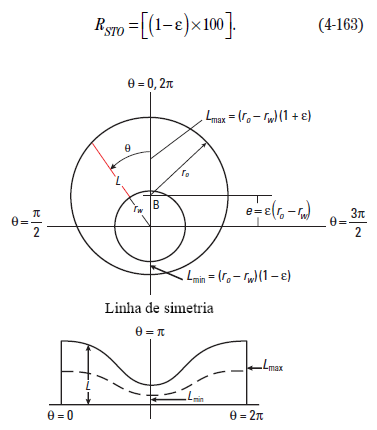
\includegraphics[width=0.75\linewidth]{img/Standoff_livro_Well.png}
	\caption{Seção transversal equivalente a um revestimento excêntrico. Fonte: \cite{Erik}}
	\label{fig:secao_transversal_equivalente_livro}
\end{figure}
Neste trabalho, consideramos simulações em que $0\% < \varsigma \leq 100\%$. Em particular, o caso em que $\varsigma$ é máximo é utilizado como modelo ideal de referência.

\subsection{Objetivos de Pesquisa}

A Matemática Computacional é capaz de propor modelos matemáticos para resolver problemas reais de alta complexidade. Aqui, procuramos dar enfoque à melhoria de processos industriais relacionados à perfuração de poços de petróleo, um tema interdisciplinar que integra diversas áreas de conhecimento, tais como matemática, física, computação e as engenharias química, mecânica e de petróleo. 

Estudar o comportamento do escoamento de colchões lavadores e sua eficiência de limpeza em diferentes configurações de poços traz benefícios para o desenvolvimento científico e tecnológico nacional, além de motivar talentos para a pesquisa. A seguir, destacamos os principais objetivos estabelecidos para a pesquisa.

\subsubsection{Objetivo Geral}

Simular numericamente o escoamento de colchões lavadores caracterizados por propriedades constituintes similares às de óleos biodegradáveis não inflamáveis que se desenvolvem durante a etapa de pré-cimentação de poços de petróleo.

\subsubsection{Objetivos Específicos}

\begin{itemize}
	\item Aplicar o método dos elementos finitos para solucionar numericamente as equações de Navier-Stokes para fluidos incompressíveis;
	\item Implementar códigos computacionais tomando como base a biblioteca FEniCS;
	\item Gerar malhas numéricas para diferentes características geométricas de poço e de espaço anular, simulando efeitos de erosão e excentricidade (\textit{standoff});
	\item Definir um parâmetro para quantificar a eficiência de varredura do escoamento em regime laminar;
	\item Analisar resultados de simulação para configurações de poço bidimensionais;
\end{itemize}

 % Revisado
\section{METODOLOGIA}

\subsection{Geração de Malhas}

Para que seja possível aplicar o método dos elementos finitos, é necessário discretizar o domínio em elementos. O domínio discretizado  chama-se malha, sobre a qual as simulações numéricas de escoamento devem ser executadas. A Fig. \ref{fig:perfuracao} ilustra a perfuração de um poço de petróleo, onde a região com hachuras em amarelo caracteriza o domínio a ser modelado.
\begin{figure}[H]
	\centering
	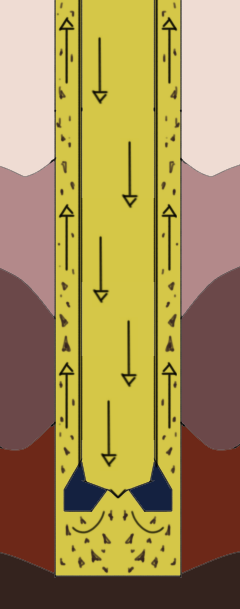
\includegraphics[scale=0.6]{img/broca.png}
	\caption[Ilustração de uma perfuração de um poço de petróleo.]{Ilustração de uma perfuração de um poço de petróleo. Fonte: autor}
	\label{fig:perfuracao}
\end{figure}


A Fig. \ref{fig:desenho_referencia_broca} é uma representação esquemática de um poço de petróleo, cuja ilustração foi utilizada como referência para criar o domínio geométrico no software AutoCad e, a partir dele, gerar o malhamento triangular. As setas representam o sentido do escoamento. As dimensões do revestimento são: 8,66 pol (aproximadamente 0,220 m) de largura e 39,37 polegadas (aproximadamente 1 m) de comprimento \cite{Rocha}. Simplificadamente, o comprimento do revestimento foi limitado a 1 m de extensão e a rugosidade na parede da formação simulada como uma interpolação por \textit{spline} de pontos definidos ``quase-aleatórios''.
\begin{figure}[H]
	\centering
	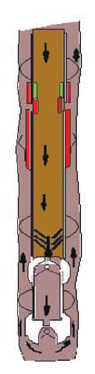
\includegraphics[scale=0.7]{img/casing1.png}
	\caption[Representação esquemática de um poço de petróleo.]{Representação esquemática de um poço de petróleo \cite{Erik}.}
	\label{fig:desenho_referencia_broca}
\end{figure}

A Fig. \ref{fig:contornos} é o resultado do desenho no AutoCad do modelo simétrico com $\varsigma$ máximo, posteriormente editada no software Paint para evidenciar o sentido do escoamento dos fluidos, bem como os contornos de entrada (\textit{inflow}) e saída (\textit{outflow}) de fluido – em verde e azul –, e também as paredes (\textit{wall}) – em marrom.
\begin{figure}[H]
	\centering
	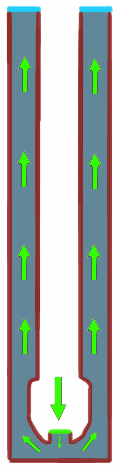
\includegraphics[scale=0.7]{img/broca_petroleo_formacao_lisa_autocad2.png}
	\caption[Representação dos contornos da malha.]{Representação dos contornos da malha. Fonte: autor.}
	\label{fig:contornos}
\end{figure}

Utilizamos o software Gmsh para gerar a malha \cite{Gmsh}. Gmsh é um programa de código aberto com o objetivo de gerar malha de elementos finitos 1D, 2D e 3D com suporte integrado a CAD. A filosofia por detrás do Gmsh é contribuir com a facilidade e rapidez na construção de uma malha. Para criar modelos, pode-se usar a interface gráfica ou a sua própria linguagem nativa por meio de \textit{scripts}. Há também uma API para as linguagens de programação C/C++, Python e Julia \cite{Gmsh}. Apesar disso, a facilidade de se trabalhar e a quantidade de recursos superior do AutoCad motivaram-nos escolhê-lo para construir o modelo. O modelo geométrico é dividido em vários elementos, tais como pontos, linhas, triângulos, quadriláteros, tetraedros e hexaedros, conectados entre si por vértices, ou nós. O Gmsh implementa vários algoritmos para gerar malhas automaticamente. As malhas em geral são não estruturadas. isto é, não existe nenhuma relação predefinida entre quaisquer dois elementos \cite{GmshDocuments}.

O Gmsh pode ler muitos tipos de arquivos. Um deles é o formato IGES, exportável pelo AutoCad. Portanto, para que haja integração entre o Gmsh e o AutoCad, trabalhamos com arquivos do tipo IGES. Normalmente, é útil combinar alguns elementos geométricos em grupos com o objetivo de definir propriedades matemáticas, tais como domínio, condições de contorno, funcionais ou materiais. Esse agrupamento pode ser feito no módulo \textit{Geometry} do Gmsh através do estabelecimento de "grupos físicos".

Para as malhas consideradas aqui, definimos 4 grupos físicos: \texttt{inflow}, \texttt{outflow}, \texttt{wall} e \texttt{flow}. Como já dissemos, o primeiro e o segundo grupo correspondem à entrada e saída de fluido. As paredes do poço, a saber, a formação rochosa nua, bem como as paredes do revestimento são tratadas pela condição de não escorregamento (\textit{no-slip}), onde a velocidade é assumida nula. Por fim, o interior do domínio, \texttt{flow}, é tratado como uma superfície física. Todas as malhas são não estruturadas e compostas de elementos triangulare com refinamento adaptativo na região de \texttt{inflow} próxima à sapata, conforme mostra a Fig. \ref{fig:malha_A_B}. Como fase final, exportamas as malhas no formato \texttt{.msh} para, em seguida, serem processadas no \textit{solver} da biblioteca FEniCS. 

%As simulações numéricas foram realizadas para diferentes tipos de geometria de poços, casos em que a formação é lisa e casos em que há um certo grau de rugosidade. Também são simulados casos de Standoff menor que 100\%, isto é, o revestimento não está perfeitamente centralizado, como foi explicado no capítulo sobre Standoff. Após as simulações numéricas, são comparados a eficiência do colchão lavador, nas diferentes geometrias de poço, por um parâmetro de eficiência de limpeza.

Consideramos 4 modelos, aqui denominados $A_1$, $A_2$, $B_1$ e $B_2$, cujas dimensões são iguais, com 1 metro de altura e 0.22 metros de comprimento, as condições iniciais e de contorno são idênticas. As propriedades do fluido simulado também são as mesmas para todas as geometrias, assim como os parâmetros de simulação. Os modelos $A$ possuem paredes lisas, ao passo que os modelos $B$ admitem rugosidades. Para os modelos $A_1$ e $B_1$, $\varsigma = 100\%$; 
para $A_2$ e $B_2$, $\varsigma < 100\%$. As malhas $A$ são representadas na figura Figs. \ref{fig:malha_A_B} com expansão da região da base do poço. As malhas $B$ são representadas na Fig.
\ref{fig:malha_C_D} também com expansão da região da base do poço, ilustrando as diferentes malhas utilizadas.
\begin{figure}[H]
	\centering
	\begin{subfigure}[b]{0.1\linewidth}
		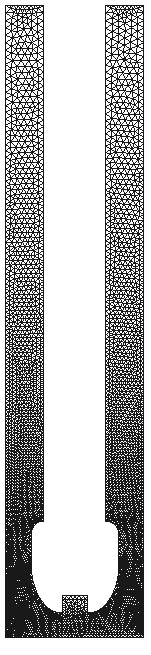
\includegraphics[width=\linewidth]{img/lisa.png}
	\end{subfigure}	
	\quad
	\quad
	\quad
	\quad
	\quad
	\begin{subfigure}[b]{0.1\linewidth}
		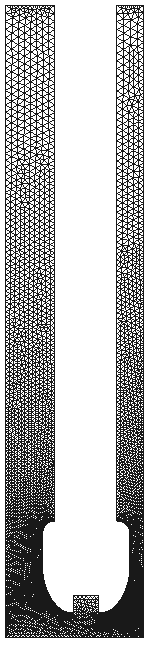
\includegraphics[width=\linewidth]{img/lisa_standoff.png}
	\end{subfigure}
	\\
	\begin{subfigure}[b]{0.3\linewidth}
		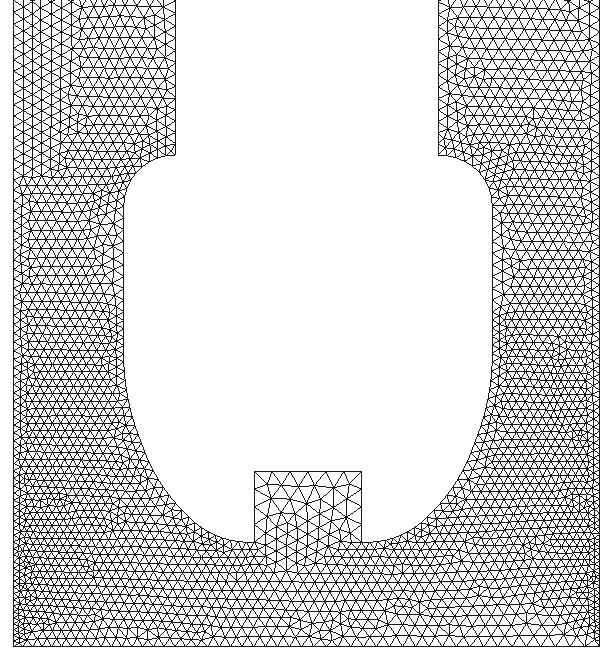
\includegraphics[width=\linewidth]{img/lisa_sapata.png}
	\end{subfigure}
	\quad
	\quad
	\quad
	\quad
	\quad
	\begin{subfigure}[b]{0.3\linewidth}
		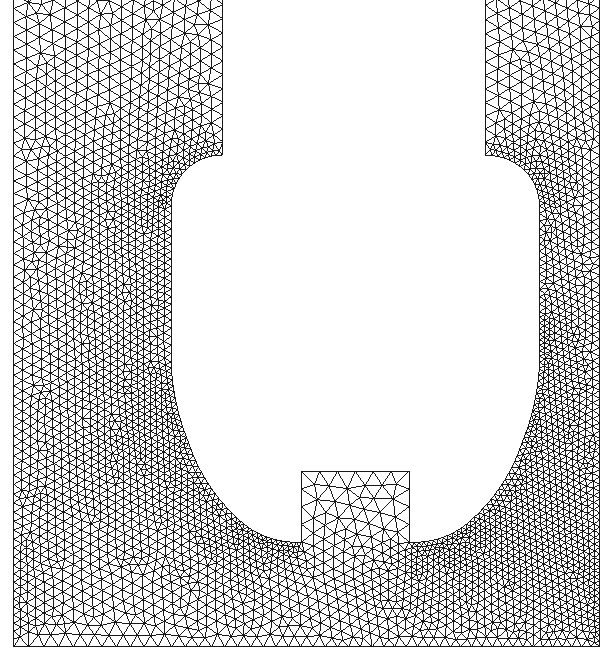
\includegraphics[width=\linewidth]{img/lisa_standoff_sapata.png}
	\end{subfigure}

	\caption[Malhas da configuração $A$: anular e sapata.]{Malhas da configuração $A$: anular e sapata. Fonte: autor.}
	\label{fig:malha_A_B}
\end{figure}

\begin{figure}[H]
	\centering
	\begin{subfigure}[b]{0.1\linewidth}
		\includegraphics[width=\linewidth]{img/rugosa.png}
	\end{subfigure}
	\quad
	\quad
	\quad
	\quad
	\quad
	\begin{subfigure}[b]{0.1\linewidth}
		\includegraphics[width=\linewidth]{img/rugosa_standoff.png}
	\end{subfigure}
	\\
	\begin{subfigure}[b]{0.3\linewidth}
		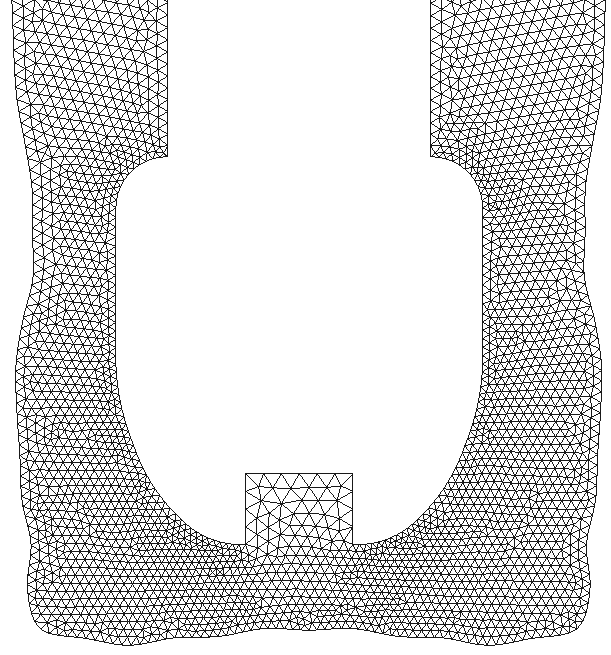
\includegraphics[width=\linewidth]{img/Rugosa_sapata.png}
	\end{subfigure}
	\quad
	\quad
	\quad
	\quad
	\quad
	\begin{subfigure}[b]{0.3\linewidth}
		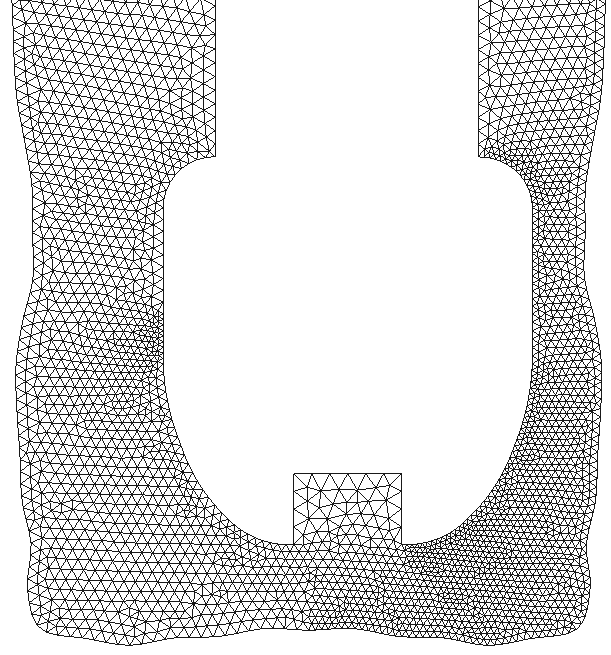
\includegraphics[width=\linewidth]{img/Rugosa_standoff_sapata.png}
	\end{subfigure}
	\caption[Malhas da configuração $B$: anular e sapata.]{Malhas da configuração $B$: anular e sapata. Fonte: autor.}
	\label{fig:malha_C_D}
\end{figure}
\noindent A Tab. \ref{tab:Geo_Valor_Standoff} resume os principais parâmetros de malha e a taxa de \textit{standoff} considerados para cada modelo. Onde $n_{elem}$, $n_{ver}$ e $n_{nos}$ é o número de elementos, de vértice e de nós da malha, respectivamente.
\begin{table}[h!]
    \centering
    \caption{Principais parâmetros de malha.}
    \begin{tabular}{ccccc}
    \hline
    modelo & $n_{elem}$ & $n_{ver}$ & $n_{nos}$ & $\varsigma$ \\
    \hline
    $A_1$ & 12520 & 6698 & 44828 & 100\% \\
    $A_2$ & 12986 & 6931 & 40458 & 50\% \\
    $B_1$ & 14706 & 7810 & 53278 & 100\% \\
    $B_2$ & 14550 & 7732 & 52654 & 50\% \\
    \hline
    \end{tabular}
    \label{tab:Geo_Valor_Standoff}
\end{table}

foi utilizado elementos triangulares de Taylor-Hood \cite{Taylor} com interpolação quadrática para a velocidade e interpolação linear para a pressão. Esses elementos são denotados como P2P1. Além de estáveis, esses elementos também convergem quadraticamente. Cada componente de velocidade será caracterizada por 6 nós enquanto a pressão será caracterizada por 3 nós Fig. \ref{fig:elements}

\begin{figure}[H]
	\centering
	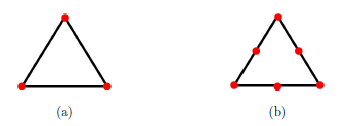
\includegraphics[scale=1]{img/elements.png}
	\caption[Representação dos contornos da malha.]{Elementos de triângulo linear e quadrático. A figura (a) corresponde aos elementos lineares de pressão e a figura (b) corresponde aos elementos quadráticos para cada componente da velocidade. Fonte: \cite{Cornthwaite}}
	\label{fig:elements}
\end{figure} %-- rev
\subsection{A Biblioteca FEniCS}

FEniCS é uma ferramenta computacional de código aberto que tem por objetivo a resolução de equações diferenciais parciais (EDPs). O FEniCS oferece rapidez para traduzir modelos físico-matemáticos em códigos de elementos finitos escritos nas linguagens de programação Python e C++ \cite{Fenics}. No programa estão implementadas a biblioteca fundamental  DOLFIN e outras funcionalidades especializadas. 

O DOLFIN fornece um ambiente de solução de problemas para modelos baseados em EDPs, incluindo estruturas de dados e algoritmos para malhas computacionais e abstrações de elementos finitos. O DOLFIN fornece classes para operar com matrizes, vetores, elementos diversos e espaços funcionais, entidades importantes para computação de elemento finitos. A interface foi projetada com o propósito de ser simples. Para resolver EDPs usando a interface DOLFIN, os usuários devem expressar os problemas na forma variacional usando a linguagem específica UFL \cite{Logg}. A Fig. \ref{fig:dolfin} exemplifica os componentes mais relevantes da biblioteca DOLFIN.
\begin{figure}[H]
	\centering
	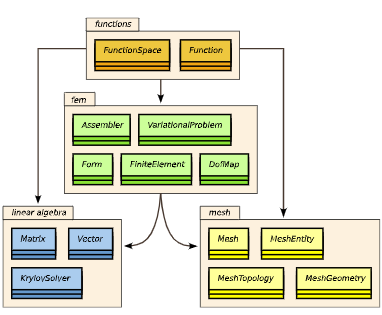
\includegraphics[scale=1]{img/esquema_dolfin.png}
	\caption[Componentes mais relevantes da biblioteca DOLFIN.]{Componentes mais relevantes da biblioteca DOLFIN \cite{Logg}.}
	\label{fig:dolfin}
\end{figure} %-- rev
\subsection{Equações de Navier Stokes}
\label{subsec:nseq}

As equações de Navier Stokes (ENS) descrevem o movimento de fluidos viscosos. Estas equações foram derivadas originalmente na década de 1840 por Claude-Louis Navier e George Gabriel Stokes com base nas leis de conservação de massa, momento linear e energia. Elas permitem determinar os campos de pressão e de velocidade em um determinado escoamento \cite{WOLFRAM}. As ENS podem ser utilizadas para modelar correntes oceânicas, escoamentos em dutos, escoamentos externos sobre aerofólios e aeronaves, hemodinâmica, entre outras aplicações \cite{Elias}.

Assumiremos neste trabalho que os fluidos escoantes são incompressíveis. Assim, consideraremos a equação da quantidade de movimento escritas na seguinte forma:
\begin{eqnarray}
	\rho \left( \dfrac{\partial \boldsymbol{u}}{\partial t} + \boldsymbol{u} \cdot \nabla \boldsymbol{u} \right) + 
	\nabla \cdot \boldsymbol{\sigma} + \boldsymbol{f} &=&  \boldsymbol{0} \label{eq:NavierStokes} \\ 
		\nabla \cdot \boldsymbol{u} &=& 0 \label{eq:NavierStokesB},
\end{eqnarray}
onde $\rho$ é a massa específica, $\boldsymbol{u}$ a velocidade, $t$ o tempo, $p$ a pressão e $\boldsymbol{f}$ a força de corpo por unidade de volume, a ser especificada adiante. Chamado de tensor de tensões de Cauchy, $\boldsymbol{\sigma}$ relaciona-se à pressão pela equação constitutiva para fluidos newtonianos dada por
\begin{equation}
\label{eq:sigma}
	\boldsymbol{\sigma} = 2 \mu \left ( \boldsymbol{u} \right ) - p\boldsymbol{I},
\end{equation}
onde $\boldsymbol{I}$ é o tensor identidade. As tensões cisalhantes e a taxa de deformação em fluidos newtonianos
relacionam-se de modo linear pela constante de proporcionalidade $\mu$, a viscosidade cinemática. O tensor de deformação $\boldsymbol{\epsilon}$ é dado por \cite{MOLON}:
\begin{equation}
\label{eq:Epsilon}
	\boldsymbol{\epsilon} = \frac{1}{2}(\nabla \boldsymbol{u} + \nabla \boldsymbol{u}^{T}).
\end{equation}

Tratando a força de corpo como a gravidade, isto é, $\boldsymbol{f} = \rho \boldsymbol{g}$, a substituição das Eqs. \eqref{eq:sigma} e \eqref{eq:Epsilon} na Eq. \eqref{eq:NavierStokes} permite-nos reescrever a equação da quantidade de movimentos como as ENS:
\begin{eqnarray}
	\rho \left( \dfrac{\partial \boldsymbol{u}}{\partial t} + \boldsymbol{u} \cdot \nabla \boldsymbol{u} \right) -
	\nabla p +
	\nabla \cdot 
	[ \mu ( \nabla \boldsymbol{u} + \nabla \boldsymbol{u}^{T}) ] 
	+ \rho \boldsymbol{g} &=& \boldsymbol{0} \label{eq:NavierStokes} \\ 
	\nabla \cdot \boldsymbol{u} &=& 0,
\end{eqnarray}
tendo em vista que $\nabla \cdot p\boldsymbol{I} = \nabla p$. %-- rev
\subsubsection{Formulação Variacional e Discretização das Equações}

A formulação padrão de Galerkin para as ENS incompressíveis, baseada em polinômios interpoladores de mesma ordem para velocidade e pressão, apresenta instabilidades. Portanto, consideramos neste trabalho espaços de elementos finitos do tipo Taylor-Hood (P2/P1) para a discretização espacial, com polinômios interpoladores quadráticos para a velocidade e lineares para a pressão, além de um método de projeção \cite{CHORIN} conhecido como \emph{Esquema de Correção Incremental da Pressão}, ou IPCS, do inglês \emph{Incremental Pressure Correction Scheme} \cite{Goda}.

A seguir, explicamos brevemente a formulação variacional, bem como a discretização temporal associadas às ENS descritas 
na subseção \ref{subsec:nseq}. Detalhes podem ser encontrados em \cite{Langtangen}. Primeiramente, definimos o produto interno genérico
\begin{equation}
\langle v,w \rangle_{\Phi} = \int_{\Phi} v w \,d\Phi,
\end{equation},
para funções contínuas $v$ e $w$ definidas em $\Phi$. Neste texto, $\Phi = \Omega$ representa o interior do domínio onde as ENS são resolvidas e $\Phi = \partial \Omega$ representa o contorno.

Para estabelecer a forma variacional para as ENS, algumas hipóteses matemáticas devem ser feitas sobre os campos de velocidade e pressão, entre elas a de continuidade, variação limitada e integrabilidade. Em linhas gerais, devemos buscar uma solução aproximada para as incógnitas $\boldsymbol{u}$ e $p$ a partir de uma forma ``enfraquecida'' que é obtida por meio de integrais ponderadas. 

Escolhendo-se funções $\boldsymbol{v}$ e $q$, a primeira vetorial e a segunda escalar, para agirem como funções de ponderação, multiplicamos as Eqs. \eqref{eq:NavierStokes} e \eqref{eq:NavierStokes}, respectivamente, por $\boldsymbol{v}$ e $q$. Após integração por partes e algumas operações algébricas, chegamos à forma compacta 
\begin{align}
\label{eq:velocidadetentativa}
	\langle \rho (\boldsymbol{u}^*-\boldsymbol{u}^n)/\Delta t, \boldsymbol{v} \rangle_{\Omega} 
	+ \langle \rho \boldsymbol{u}^n \cdot \nabla \boldsymbol{u}^n, \boldsymbol{v} \rangle_{\Omega} 
	+ \langle \sigma (\boldsymbol{u}^{n + \frac{1}{2}}, 	p^n),\boldsymbol{\epsilon}(\boldsymbol{v}) \rangle_{\Omega} + \nonumber \\
	- \langle \boldsymbol{n}p^n,\boldsymbol{v} \rangle _ {\partial \Omega} 
	+ \langle \mu \boldsymbol{n} \nabla \boldsymbol{u}^{n + \frac{1}{2}},\boldsymbol{v} \rangle_{\partial \Omega} 
	+ \langle \rho^{n+1}, \boldsymbol{v} \rangle_{\partial \Omega}
	=\boldsymbol{0},
\end{align}
que caracteriza a forma variacional já discretizada no tempo para um passo de tempo $\Delta t$. A Eq. \eqref{eq:velocidadetentativa} é, além disso, o primeiro passo do método ICPS, em que a velocidade tentativa $\boldsymbol{u}^*$ é uma estimativa que não obedece à restrição de divergência nula dada pela Eq.\eqref{eq:NavierStokesB}.

A notação $\boldsymbol{u}^{n+\frac{1}{2}}$ sugere uma aproximação implícita para $\boldsymbol{u}$ avaliada no ponto médio temporal, ou seja,
$$\boldsymbol{u}^{n+\frac{1}{2}} \approx (\boldsymbol{u}^n + \boldsymbol{u}^{n+1})/2.$$

No segundo passo do método IPCS, calculamos a estimativa para a pressão resolvendo uma equação tipo Poisson usando a velocidade tentativa então calculada
\begin{equation}\label{eq:pressure}
	\langle \nabla p^{n+1} ,\nabla q \rangle_{\Omega} 
	= \langle \nabla p^n , \nabla q\rangle_{\Omega} 
	- \Delta t^{-1} \langle \nabla \cdot \boldsymbol{u}^{*},q \rangle_{\Omega},
\end{equation}

Agora que temos a nova pressão, basta calcular a velocidade corrigida $\boldsymbol{u}^{n+1}$, tal que $\nabla \cdot \boldsymbol{u}^{n+1} = 0$. Este é o terceira e último passo do método ICPS:
\begin{equation}\label{eq:corrected_velocity}
	\langle \boldsymbol{u}^{n+1}, \boldsymbol{v} \rangle_{\Omega} 
	= \langle \boldsymbol{u}^*, \boldsymbol{v} \rangle_{\Omega} 
	- \Delta t \langle \nabla (p^{n+1}-p^n), \boldsymbol{v} \rangle _{\Omega}.
\end{equation}
Em suma, para cada passo de tempo no processo iterativo de solução das ENS, as 3 equações acima são resolvidas por um processo de \textit{splitting} \cite{Langtangen}. 

%\textcolor{red}{Qual formulação utilizar para resolver o problema, exemplo: Arbitrary Lagrangian Eulerian Variational Multi-scale formulation (ALE-VMS), petrov-galerkin,PSPG}

%\textcolor{red}{O tamanho do passo de tempo é de suma importância em problemas que possuem dependência temporal, pois este influencia na solução a ser obtida, no tempo computacional, entre outros fatores. A fim de obter um passo de tempo adequado, foi utilizado o controlador Proporcional-Integral-Diferencial (PID) (VALLI; CAREY; COUTINHO, 2002) para as equações de Navier-Stokes}

%Estas equações serão solucionadas utilizando a ferramenta FEniCS, para tal, deve-se seguir os seguintes passos.\cite{Logg}
%\begin{enumerate}
	%\item Identificar o PDE e as condições de contorno
	%\item Reformular o problema de PDE como um problema variacional
	%\item Construir um programa Python onde as fórmulas do problema variacional são codificadas, junto com as definições dos dados de entrada como $f$, $u_0$ e uma malha para $\Omega$ em (\ref{eq:NavierStokes}).
	%\item Adicionar declarações no programa para resolver o problema variacional, computando quantidades derivadas, como $ \nabla \boldsymbol{u} $, e visualizando os resultados.
%\end{enumerate}

%Será discorrido cada um desses itens. Começando pelo primeiro item, o problema de PDE em questão é o já mencionado acima:\ref{eq:NavierStokes}, sendo assim, para completar o primeiro item da lista, as condições de contorno, é necessário entender melhor o domínio em que o problema reside. %-- rev
\subsubsection{Implementação Computacional}

\lstset{caption={Implementação computacional}}

A implementação computacional das equações discretas foi realizada na linguagem Python. A seguir, inserimos porções compactas do código aplicado. A versão completa está disponível no Apêndice. Após importar todas as bibliotecas necessárias, importar a malha que foi gerada via Gmsh como .msh como mostra o cód no apendice. As funções \texttt{create\_mesh} e \texttt{mvc\_mf}, servem para extrair os grupos físicos definidos no Gmsh, para identificação direta pelo FEniCS.
\begin{comment}

    \begin{lstlisting}[title=\phantom{}]
    def create_mesh(mesh, cell_type, prune_z=False):
        cells = mesh.get_cells_type(cell_type)
        cell_data = mesh.get_cell_data("gmsh:physical", cell_type)
        out_mesh = mio.Mesh(points=mesh.points, 
                   cells= {cell_type: cells},
                   cell_data={"name_to_read": [cell_data]})
        if prune_z:
            out_mesh.prune_z_0()
        return out_mesh
    
    def mvc_mf(mesh_from_file):
        line_mesh = create_mesh(mesh_from_file, 
                    "line", prune_z=True)
        mio.write("facet_mesh.xdmf", line_mesh)
        triangle_mesh = create_mesh(mesh_from_file,"triangle",
                        prune_z=True)
        mio.write("mesh.xdmf", triangle_mesh)
        mesh = Mesh()
    
        with XDMFFile("mesh.xdmf") as infile:
            infile.read(mesh)
            mvc = MeshValueCollection("size_t", mesh, 2)
    
        with XDMFFile("facet_mesh.xdmf") as infile:
            infile.read(mvc, "name_to_read")
            mf = MeshFunction("size_t", mesh, mvc)
        
        return mesh, mvc, mf
    \end{lstlisting}
    
\end{comment}

A partir da malha importada e da identificação dos grupos físicos, as propriedades de fluido, os parâmetros de simulação, tempo, quantidade de iteração, assim como as condições de contorno e iniciais podem ser definidos na função \texttt{dados\_entrada}.
\begin{comment}

\begin{lstlisting}[title=\phantom{}]
def dados_entrada(type_fluido):
    dados_problema = {'diametro_saida':40,
                      'Tempo': 10,
                      'grav':-9.85,
                      'num_steps': 40000}
                      
    dados_problema['velocidade_fluido_inflowX'] = 0
    dados_problema['velocidade_fluido_inflowY'] =
    -1000*(500*0.0381)/(900*0.04)
    dados_problema['dt'] =
    int(dados_problema['Tempo'])/int(dados_problema['num_steps'])
    
    colchao_lavador = {
        'nome': "colchao_lavador",
        'viscosidade': 38.1,
        'densidade': 0.000900
    }

    dados_fluidos = [colchao_lavador]
    return dados_fluidos[type_fluido - 1], dados_problema
\end{lstlisting}
    
\end{comment}

A função \texttt{def} descreve o modelo matemático das equações de Navier-Stokes. As linhas 5-7 definem a velocidade inicial e as linhas 9-14 as condições de contorno. %Como há uma condição de não deslizamento nas paredes da formação e no revestimento, então a velocidade é definida como nula na linha 12. Na linha 11 é definido a pressão no contorno da saída como nula.
As linhas 35-39 referem-se às equações \ref{eq:Epsilon} e \ref{eq:sigma}, que representam, respectivamente, o tensor de tensões de Cauchy e o tensor de deformação. 

Depois de importar a biblioteca, definir os dados do problema, importar a malha, informar as condições de contorno, implementa-se o método IPCS. As linhas 41-48 referem-se às equações \ref{eq:velocidadetentativa}, \ref{eq:pressure} e \ref{eq:corrected_velocity}. As linhas 50-52 realizam a correção da pressão. Com a pressão corrigida, calcula-se a velocidade corrigida.

\begin{lstlisting}[title=\phantom{}]
def modelo(mesh, dados_problema,dados_fluidos, cfl, mf):
    V = VectorFunctionSpace(mesh, 'P', 2) 
    Q = FunctionSpace(mesh, 'P', 1)  
    
    inflow_profile = ('0' + 
    str(dados_problema['velocidade_fluido_inflowX']), '0' + 
    str(dados_problema['velocidade_fluido_inflowY']))
    
    bcu_inflow = DirichletBC(V, Expression(inflow_profile, 
    degree=2), mf, 1)
    bcp_outflow = DirichletBC(Q, Constant(0), mf, 2)
    bcp_paredes = DirichletBC(V, Constant((0, 0)), mf, 3)
    bcu = [bcu_inflow, bcp_paredes]  
    bcp = [bcp_outflow]  
    
    u = TrialFunction(V)
    v = TestFunction(V)
    p = TrialFunction(Q)
    q = TestFunction(Q)
    
    u0 = Function(V)
    u_ = Function(V)
    p_n = Function(Q)
    p_ = Function(Q)
    
    U = 0.5 * (u0 + u)
    n = FacetNormal(mesh)
    f = Constant((0, dados_problema['grav']))
    k = Constant(cfl['dt'])
    
    viscosidadeCinematica =
        Constant(dados_fluidos['viscosidade'])
    massa_especifica =
        Constant(dados_fluidos['massa_especifica'])
    beta = 1
    
    def epsilon(u):
        return (1 / 2) * (nabla_grad(u) + nabla_grad(u).T)
    
    def sigma(u, p, viscosidadeCinematica):
        return 2 * viscosidadeCinematica \
        * epsilon(u) - p * Identity(len(u))
    
    F1 = (1.0 / k) * inner(u - u0, v) * df.dx \
        + inner(grad(u0) * u0, v) * df.dx \
        + inner(sigma(U, p_n, viscosidadeCinematica), 
        epsilon(v)) * df.dx \
        + inner(p_n * n, 
        v) * df.ds \
        - beta * viscosidadeCinematica * inner(grad(U).T * n, 
        v) * df.ds \
        - viscosidadeCinematica * inner(f, v) * df.dx
    a1 = lhs(F1)
    L1 = rhs(F1)
    
    a2 = inner(grad(p), grad(q)) * df.dx
    L2 = inner(grad(p_n), grad(q)) * df.dx \
        - (1.0 / k) * div(u_) * q * df.dx
    
    a3 = inner(u, v) * df.dx
    L3 = inner(u_, v) * df.dx \
        - k * inner(grad(p_ - p_n), v) * df.dx
    
    A1 = assemble(a1)
    A2 = assemble(a2)
    A3 = assemble(a3)
    
    [bc.apply(A1) for bc in bcu]
    [bc.apply(A2) for bc in bcp]
    
    modelo = {'A1': A1,
    	'A2': A2,
    	'A3': A3,
    	'bcu': bcu,
    	'bcp': bcp,
    	'cfl': cfl,
    	'L1': L1,
    	'L2': L2,
    	'L3': L3,
    	'u_': u_,
    	'p_': p_,
    	'u0': u0,
    	'p_n': p_n}
    
    return modelo
\end{lstlisting}

A função \texttt{solucao} soluciona as equações para cada passo de tempo dentro de uma laço de repetição. As linhas 4-6 aplicam as condições iniciais de contorno às matrizes. Nas linhas 8-19, resolve-se o método IPCS.

\begin{lstlisting}[title=\phantom{}]

def solucao(modelo):
    passos = 0
    t = 0
    for n in tqdm(range(modelo['cfl']['num_steps'])):
        [bc.apply(modelo['A1']) for bc in modelo['bcu']]
        [bc.apply(modelo['A2']) for bc in modelo['bcp']]
        
        b1 = assemble(modelo['L1'])
        [bc.apply(modelo['A1'], b1) for bc in modelo['bcu']]
        solve(modelo['A1'], modelo['u_'].vector(), b1, 'bicgstab',
        'hypre_amg')
        
        b2 = assemble(modelo['L2'])
        [bc.apply(b2) for bc in modelo['bcp']]
        solve(modelo['A2'], modelo['p_'].vector(), b2, 'bicgstab',
        'hypre_amg')
        
        b3 = assemble(modelo['L3'])
        solve(modelo['A3'], modelo['u_'].vector(), b3, 'cg', 'sor')
        
        if n \% 200 == 0:
            pvd_file = File('velocidade-{0}.pvd'.format(passos))
            pvd_file << modelo['u_']
            pvd_file = File('pressao-{0}.pvd'.format(passos))
            pvd_file << modelo['p_']
            passos = passos + 1
        
        modelo['u0'].assign(modelo['u_'])
        modelo['p_n'].assign(modelo['p_'])
        t = t + modelo['cfl']['dt']
    return modelo
\end{lstlisting} % -- rev -->
\subsection{Quantificação da Eficiência de Varrido}
    
A fim de realizar a quantificação do efeito das erosões na parede da formação sobre a frente de propagação do escoamento, desenvolvemos um método comparativo de eficiência. Comumente, a determinação da eficiência de colchões lavadores depende do cálculo de áreas ``molhadas'' do espaço anular que são ocupadas pelos colchões em relação à área total disponível. Há diversas fórmulas na literatura para conceitos próximos, tais como, \emph{eficiência de limpeza}, \emph{eficiência de deslocamento} \cite{Monica} e \emph{eficiência de remoção} \cite{ARANHA}. Aqui, adotaremos o termo \emph{eficiência de varrido} para um coeficiente adimensional que quantifica o desvio relativo da vazão aproximada do escoamento de um colchão lavador por um espaço anular em uma configuração de paredes livres de erosão para com a configuração de paredes erodidas. A seguir, descrevemos a construção teórica do parâmetro de eficiência que empregaremos.  

Consideremos o domínio do espaço anular descrito no plano cartesiano $x,y$ com $y$ orientado positivamente para cima (Fig. \ref{fig:eta-esquema}). A parede da formação e do tubo de revestimento na configuração lisa (modelo $A$) possui extensão vertical invariável e está limitada na porção esquerda (direita) pelo intervalo $[x_0^E,x_f^E]$ ($[x_0^D,x_f^D]$). Na configuração erodida, assume-se que a parede da formação varia lateralmente ao longo da extensão vertical por pequenas perturbações de acordo com uma função $\xi^E(y)$ ($\xi^D(y)$) que descreve um perfil de contorno médio em relação a $x = x_0^E$ ($x = x_f^D$) fixado.
\begin{figure}[h]
	\centering
	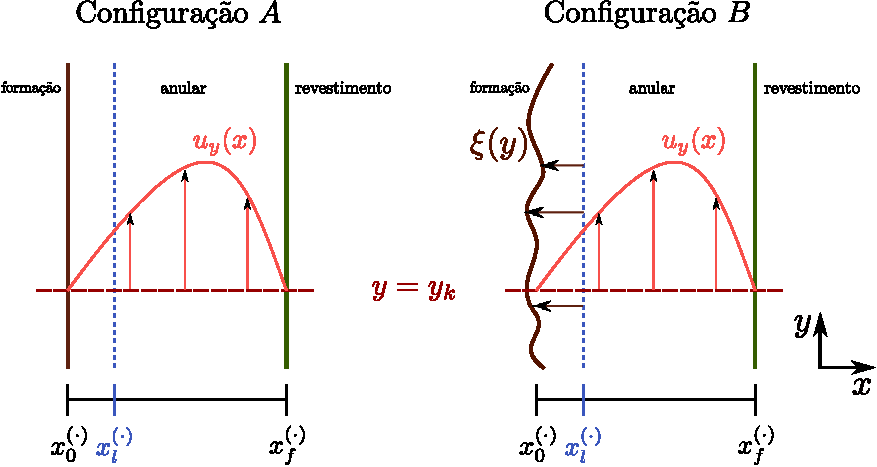
\includegraphics[scale=.8]{img/eta-esquema.pdf}
	\caption{Esquema representativo para cálculo de vazões nas configurações de poço não erodido ($A$) e poço erodido ($B$). Fonte: Autor.}
	\label{fig:eta-esquema}
\end{figure}

No segmento $[x_0^E,x_f^E]$ ($[x_0^D,x_f^D]$), escolhemos $x_l^E$ ($x_l^D$) como um ponto que particiona a porção anular esquerda em dois subsegmentos
tais que $[x_0^E,x_f^E]$ = $[x_0^E,x_l^E] \cup (x_l^E,x_f^E]$ ($[x_0^D,x_f^D]$ = $[x_0^D,x_l^D] \cup (x_l^D,x_f^D]$), onde $l$ indica que $x_l^E$ ($x_l^D$) está afastado de
$x_f^E$ ($x_f^D$) aproximadamente por um comprimento de $l$\% da largura da porção anular esquerda (direita).

Definimos
\begin{eqnarray}
    Q_p^{(q)}(y_k) &=& \int_{x_0^q}^{x_f^q} u_y(x) \, dx \, \Bigg|_{y = y_k}, \ \ \ q = D,E \ \ \text{e} \label{eq:vazaoA}\\
    Q_{p,l}^{(q)}(y_k) &=& \int_{x_l^q}^{x_f^q} u_y(x) \, dx \, \Bigg|_{y = y_k}, \ \ \ q = D,E, \label{eq:vazaoB}
\end{eqnarray}
respectivamente, como a \emph{vazão planar total na porção anular $q$} e a \emph{vazão planar percentual na porção anular $q$} na configuração $p$ à profundidade $y = y_k$. Isto é, tais quantidades representam medidas da frente de propagação do escoamento ao longo da direção $y$, levando em conta a variação da componente $u_y$ da velocidade sobre o corte transversal (direção $x$). Quando $p = A$, as quantidades referem-se ao caso de poço não erodido; quando $p = B$, ao caso de poço erodido.

A partir das Eqs. \eqref{eq:vazaoA} e \eqref{eq:vazaoB}, definimos
\begin{equation}
    %\eta_p^{(q)}(y_k) = \dfrac{Q_p^{(q)}(y_k) - Q_{p,l}^{(q)}(y_k)}{Q^{(q)}(y_k)}, \ \ p = A,B
    \eta_l^{(q)}(y_k) = \dfrac{Q_{B,l}^{(q)}(y_k)}{Q_{A,l}^{(q)}(y_k)} \times 100\%, \ \ q = D,E
\end{equation}
como o \emph{coeficiente de eficiência de varrido efetivo a $l\%$ do revestimento} na porção anular $q$, de maneira que
\begin{equation}
    %\eta^{(q)}(y_k) = \dfrac{\eta_B^{(q)}(y_k)}{\eta_A^{(q)}(y_k)} \times 100\%
    \eta^{(q)}(y_k) = \dfrac{Q_{B}^{(q)}(y_k)}{Q_{A}^{(q)}(y_k)} \times 100\%, \ \ q = D,E
\end{equation}
é o \emph{coeficiente de eficiência de varrido total} na porção anular $q$ para a profundidade $y_k$. Nesses termos, à medida que $\eta_l^{(q)}(y_k)$ ($\eta^{(q)}(y_k)$) tende a 100\%, o efeito das erosões sobre a propagação do escoamento é praticamente desprezível; opostamente, à medida que tende a 0\%, esse efeito é considerável.

Ambos os coeficientes usam a configuração não erodida como modelo de referência para a configuração erodida, permitindo, dessa maneira, a quantificação da influência das erosões na perda de vazão planar. Entretanto, o coeficiente de eficiência de varrido efetivo captura essa influência de modo indireto através da alteração detectada no escoamento apenas na porção livre do anular. Já o coeficiente de eficiência de varrido total mede a influência diretamente.


%Este parâmetro é obtido pela equação $\eta = \frac{Q - Q{limp}}{Q_{limp}}$. Onde, $Q$ é a vazão no espaço anular e ${Q_{limp}}$ é a vazão no espaço anular sem os efeitos da parede e do revestimento, onde a velocidade é zero, como é detalhado mais adiante. 
    
%Este parâmetro é calculado para o lado esquerdo e direito individualmente e para 3 níveis de profundidade distintas das geometrias.
    
%Inicialmente é utilizado o programa Paraview para processar os dados da simulação numérica e extrair o arquivo csv que possui os dados da última iteração, um arquivo para cada nível de profundidade definido através da ferramenta plotoverline no mesmo programa. Esse arquivo pode ser exportado, após aplicar o plotoverline no nível desejado, na opção Save Data.
    
%Após isso, é implementado um código em python para leitura e processamento do arquivo CSV com o foco em calcular o parâmetro de limpeza desejado. Para fins didáticos, será detalhado o funcionamento básico do código a seguir.
    
%A linha 1 é a leitura do arquivo de dados do perfil de velocidade em CSV. Há dados em $nan$ que provêm dos pontos que não intersectam a malha, portanto faz-se necessário limpar o dataframe e resetar o index, linha 2.
    
%    \begin{lstlisting}
%    	df = pd.read_csv('linha11-y240.csv')
%    	df = df.dropna().reset_index(drop=True)
%    \end{lstlisting}
    
%A linha 1 do cód. a seguir é a componente de velocidade na direção $x$ e a linha do 2 é a componente de velocidade na direção $y$. v é o modulo da velocidade. x é o eixo x.
    
 %   \begin{lstlisting}
 %   	vx = df['f_24:0']
 %   	vy = df['f_24:1']
 %   	v = np.sqrt(vx**2 + vy**2).values
 %   	x = df['Points:0'].values
 %   \end{lstlisting}
    
%O cód. a seguir plota o perfil de velocidade em todo o eixo x
    
 %   \begin{lstlisting}
%    	plt.plot(x,v)
 %   \end{lstlisting}
    
%    \begin{figure}[H]
 %   	\centering
 %   	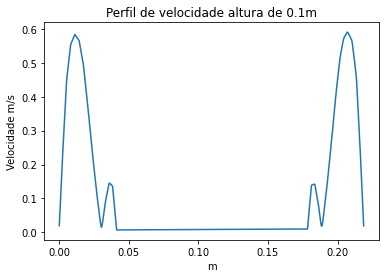
\includegraphics[scale=0.65]{img/perfil_vel/liso/perfil_velocidade_liso_100.png}
%	    \caption{Fonte: autor.}
 %   	\label{fig:perfil_velocidade_nivel_202}
 %   \end{figure}
    
%O cód. a seguir separa os dois lados onde o perfil de velocidade é diferente de zero, em outras palavras, o espaço anular esquerdo e o espaço anular direito. A imagem \ref{fig:perfil_velocidade_202_esquerdo} mostra o perfil de velocidade do lado esquerdo
    
%    \begin{lstlisting}
%    	nao_nulo_esq = np.argwhere((x < 33)).flatten()
 %   	nao_nulo_dir = np.argwhere((x > 135)).flatten()
 %   \end{lstlisting}
    
 %   \begin{figure}[H]
 %   	\centering
 %   	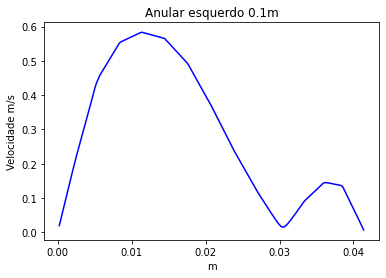
\includegraphics[scale=0.65]{img/perfil_vel/liso/perfil_velocidade_liso_esquerdo_100.png}
 %   	\caption{Fonte: autor.}
 %   	\label{fig:perfil_velocidade_202_esquerdo}
 %   \end{figure}
    
%A figura \ref{fig:/perfil_velocidade_202_esquerdo_delimitado} apresenta a eliminação do efeito de velocidade nula no contorno da formação.
    
 %   \begin{figure}[H]
 %   	\centering
 %   	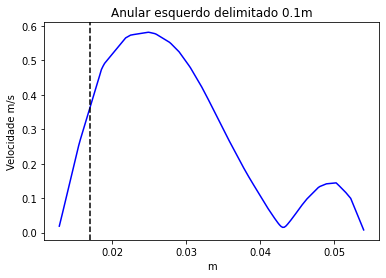
\includegraphics[scale=0.65]{img/perfil_vel/liso/perfil_velocidade_liso_esquerdo_delimitado_100.png}
%   	    \caption{Fonte: autor.}
%     	\label{fig:/perfil_velocidade_202_esquerdo_delimitado}
%     \end{figure}
    
% O cód. a seguir calcula a largura do espaço anular esquerdo e direito, $h_e$ e $h_d$ respectivamente
    
%     \begin{lstlisting}
%     	E = x[nao_nulo_esq]; D = x[nao_nulo_dir];
%     	h_e = np.max(E) - np.min(E)
%     	h_d = np.max(D) - np.min(D)
%     \end{lstlisting}
    
% O cód. a seguir calcula a área utilizando as equações $Qe = \int{he} ve dx$ e $Qd = \int{hd} vd dx$, do lado esquerdo e direito respectivamente. Para calcular é aplicado a integração numérica e regra do trapézio.
    
%     \begin{lstlisting}
%     	v_e = v[nao_nulo_esq]; v_d = v[nao_nulo_dir]
%     	Q_e = trapezoid(v_e)
%     	Q_d = trapezoid(v_d)
%     \end{lstlisting}
    
% Para calcular o parâmetro $\eta$ da eficiência de limpeza, é necessário "excluir" o efeito de velocidade nula no contorno do revestimento e da parede do poço. No espaço anular esquerdo o efeito do revestimento é do lado direto e o de parede é do lado esquerdo. No espaço anular direito, o efeito do revestimento é do lado esquerdo e o da parede é do lado direito. Foi adotado um percentual arbitrário de $10\%$ de ambos os lados do espaço anular para ser eliminado. Após isso, é necessário calcular a área no novo intervalo delimitado, ou seja, calcular a integral dos perfis de velocidade nos intervalos $[ha,hb]$ para obter $Q{limp}$
    
%     \begin{lstlisting}
%     	X = 0.1
%     	delta_e = X*h_e
%     	delta_d = X*h_d
%     	h_a = (delta_e,h_e - delta_e)
%     	h_b = (delta_d,h_d - delta_d) 
%     \end{lstlisting}
    
% Considerando apenas o lado esquerdo do espaço anular, o cálculo de $\eta_{e}$ é dado por  $\eta_{e} = \frac{Qe -	Q{limp_e}}{Q_{limp_e}}$ onde  $\eta_{e}$ é o parâmetro de limpeza do lado esquerdo, $Q{e}$ é a área do perfil de velocidade do lado esquerdo e $Q{limp_e}$ é a área do perfil de velocidade do lado esquerdo delimitado. O código a seguir representa esse cálculo 
%     \begin{lstlisting}
%     	n_e = (Q_e-Qlimpo_e)/Qlimpo_e
%     \end{lstlisting}
    
%     Esta análise acima é replicada para o lado direito do espaço anular.
 % -- rev
\section{RESULTADOS E DISCUSSÃO}

Nesta seção, apresentamos os resultados das simulações numéricas obtidas para as configurações de poço dos tipos $A$ e $B$ processados via biblioteca FEniCs e pós-processados no software Paraview. 

\subsection{Posicionamento do Problema-Base}

Os experimentos levam em consideração um único tipo de colchão lavador à base de óleo vegetal com viscosidade cinemática de 0,18 Pa.s e massa específica de 900 kg.m\textsuperscript{-3} \cite{ARANHA}. Para definir a velocidade de entrada, assumimos um diâmetro de 0,4 m para o bocal de saída de fluido no fundo de poço como comprimento de referência e $Re$ = 500, que mantém o escoamento dentro do regime laminar \cite{Lupyana}. A profundidade dos poços é assumida pequena, de modo que a aceleração da gravidade permanece fixada em 9.8 m.s\textsuperscript{-2}. A extensão do domínio na direção normal ao escoamento (largura) equivale a de um poço com 8,66 pol. (aproximadamente 0,22 m) de diâmetro. Na direção tangente ao escoamento, o domínio limita-se a 1 m de comprimento.

Consideramos $\Omega_d$ o domínio, $\Gamma_p$ o contorno da parede da formação, $\Gamma_r$ o contorno do revestimento, $\Gamma_e$ o contorno do orifício por onde o fluido é expelido e $\Gamma_s$ o contorno do anular por onde o fluido escapa. Reescrevendo as equações de Navier-Stokes de maneira compacta, podemos definir o problema de valor de contorno e inicial da seguinte forma: determinar os campos $\boldsymbol{u}$ e $p$ no espaço anular, tais que:
\begin{eqnarray}
    \label{eq:problema-abstrato}
    		\mathcal{L}[\boldsymbol{u},p;\rho,\mu,\boldsymbol{g}] &=& \boldsymbol{0} \\
    		\nabla \cdot \boldsymbol{u} &=& 0,
\end{eqnarray}
sujeito às condições de contorno e inicial
      \begin{eqnarray}
    \label{eq:problema-abstrato}
    		\boldsymbol{u}|_{\Gamma_{p}} &=& \boldsymbol{0} \\
    		%\boldsymbol{n} \cdot \nabla p|_{\Gamma_{s}} &=& 0 \\
            p|_{\Gamma_{s}} &=& 0 \\
    		\boldsymbol{u}|_{\Gamma_{e}} &=& \boldsymbol{u_0}.
    \end{eqnarray}
\subsection{Configurações do Resolvedor Numérico}

A fim de resolver os sistemas lineares, utilizamos o \textit{método do gradiente biconjugado estabilizado} (\texttt{bicgstab}) para o cálculo da velocidade tentativa e da pressão. De forma geral, o \texttt{bicgstab} utiliza menos memória que outros métodos. Para a correção de velocidade, foi utilizado o \textit{método do gradiente conjugado} \texttt{cg}. Como pré-condicionador, utilizamos o \texttt{hypre\_amg}.

%Pré-condicionadores possuem um papel fundamental na convergência dos métodos citados anteriormente. Uma vez que a taxa de convergência para a maioria dos solucionadores lineares iterativos aumenta quando o número de condição de uma matriz diminui como resultado do pré-condicionamento. Diante disso, foram selecionados pré-condicionadores adequados.

\subsection{Simulações Numéricas}

Consideramos 4 configurações de poço para as simulações: $A_1$ (anular concêntrico sem erosões); $A_2$ (anular excêntrico sem erosões); $B_1$ (anular concêntrico com erosões); $A_2$ (anular excêntrico com erosões). Para calcular o coeficiente de eficiência de varrido do colchão lavador, escolhemos 4 cotas de profundidade, a saber $y_k = \{0,1; 0,3; 0,7; 1.0\}$, assim retornando os respectivos valores $\eta(y_k)$, para $k=1,2,3,4$ para as porções esquerda e direita do anular. O \textit{loop} temporal considerou um passo de tempo $\Delta t = 0.00025$ com 40 mil iterações. Cada simulação durou, em média, 3 horas, em um computador com processador Intel Core i5 8a. geração e 8 GB RAM.

\subsubsection{Configurações sem Erosões}

Considerando a geometria sem nenhum tipo de erosão na parede do poço e com valor de \textit{standoff} 100\% $A_1$, é possível observar na Fig. \ref{fig:perfil_velocidade_liso_saida_paraview_10s} o efeito de escoamento parabólico na saída do espaço anular.
\begin{figure}[H]
        \centering
    	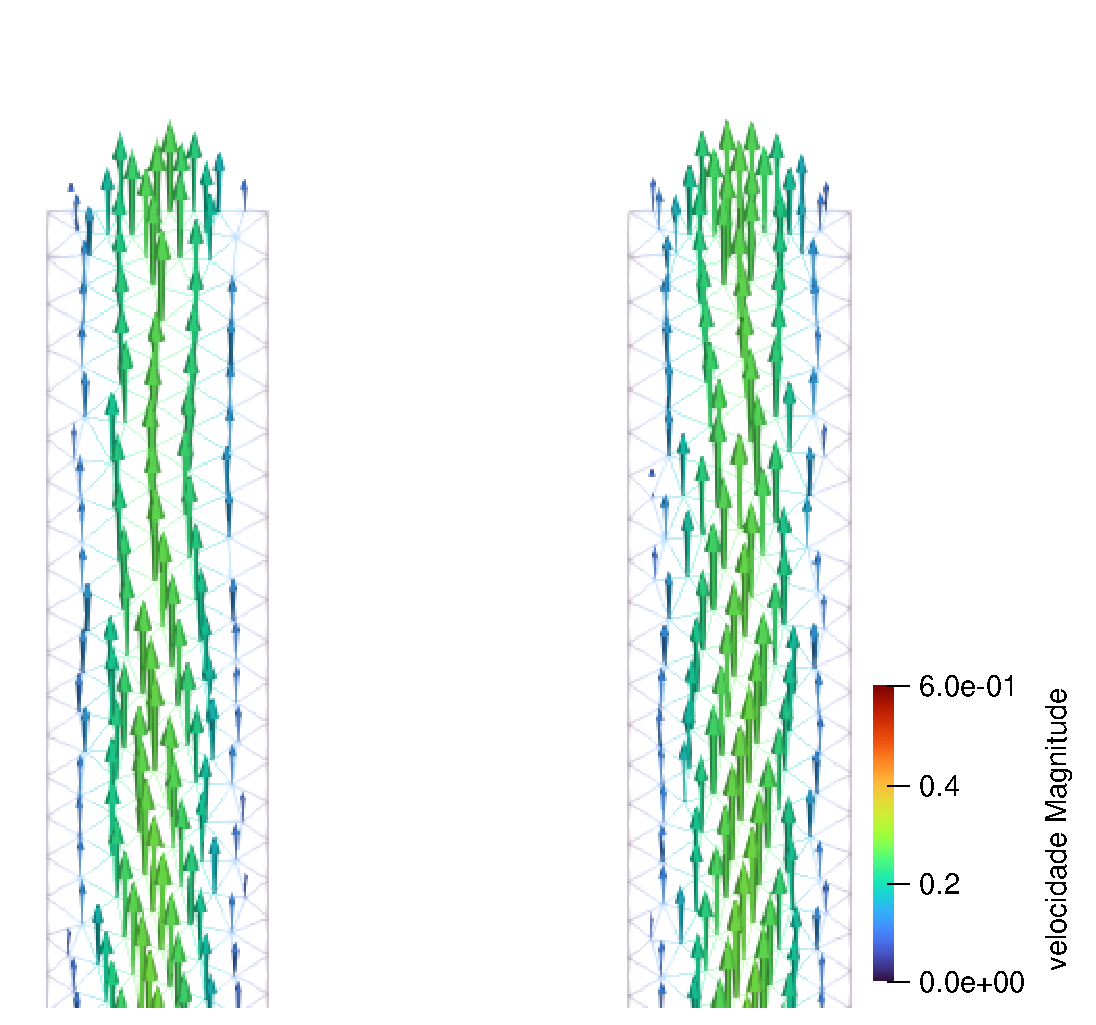
\includegraphics[scale=0.5]{img/perfil_vel/liso/perfil_de_vel_saida_paraview.eps}
    	\caption[Campo de velocidade na saída do espaço anular no tempo de 10s na geometria $A_1$.]{Campo de velocidade na saída do espaço anular no tempo de 10s na geometria $A_1$. Fonte: autor}
    	\label{fig:perfil_velocidade_liso_saida_paraview_10s}
\end{figure}
    
A Fig. \ref{fig:perfil_velocidade_liso_sapata_paraview_0_5s} é o perfil de velocidade no tempo de 0,5 segundo. Podemos observar a simetria do escoamento por se tratar de um caso com excentricidade nula. 
\begin{figure}[H]
        \centering
        \begin{subfigure}[b]{0.42\linewidth}
    		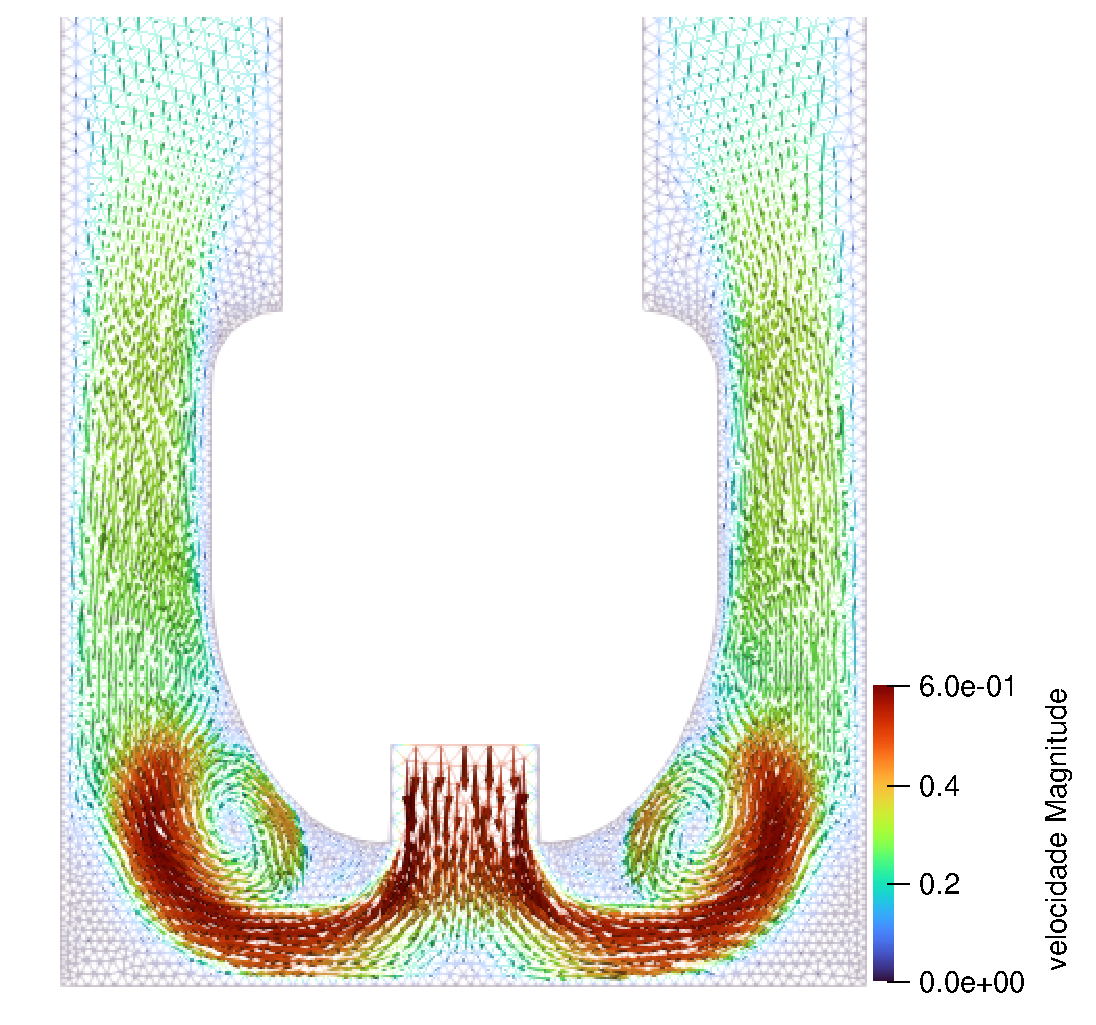
\includegraphics[width=\linewidth]{img/perfil_vel/liso/perfil_de_vel_sapata_paraview_0.5s.eps}
    	\end{subfigure}
    	\begin{subfigure}[b]{0.42\linewidth}
    		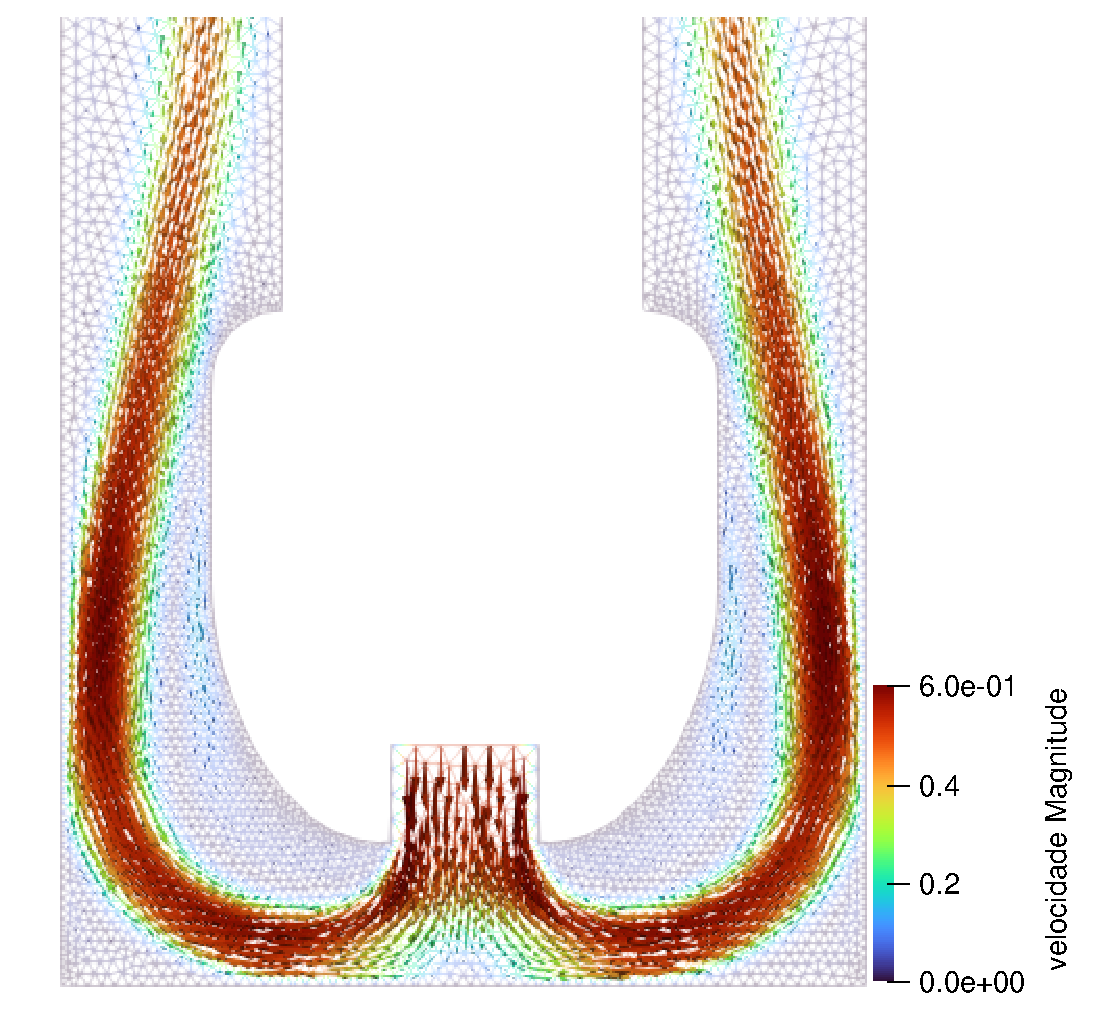
\includegraphics[width=\linewidth]{img/perfil_vel/liso/perfil_de_vel_sapata_paraview_10s.eps}
    	\end{subfigure}
    	
    	\caption{Campo de velocidade na sapata no tempo de 0.5s e 10s na geometria $A_1$. Fonte: autor}
    	\label{fig:perfil_velocidade_liso_sapata_paraview_0_5s}
\end{figure}
    
 A Fig. \ref{fig:perfil_velocidade_liso} mostra o perfil de velocidade na geometria $A_1$ para os 4 níveis distintos.
\begin{figure}[H]
    	\begin{subfigure}[b]{0.42\linewidth}
    		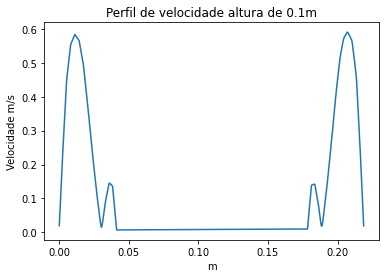
\includegraphics[width=\linewidth]{img/perfil_vel/liso/perfil_velocidade_liso_100.png}
    	\end{subfigure}
    	\begin{subfigure}[b]{0.42\linewidth}
    		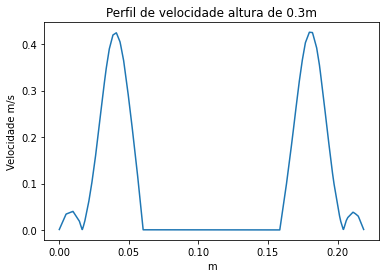
\includegraphics[width=\linewidth]{img/perfil_vel/liso/perfil_velocidade_liso_300.png}
    	\end{subfigure}
    	\\
    	\begin{subfigure}[b]{0.42\linewidth}
    		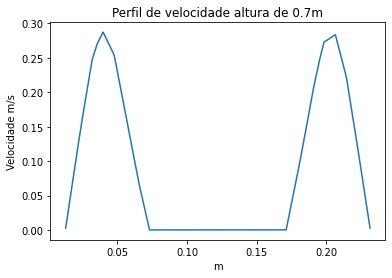
\includegraphics[width=\linewidth]{img/perfil_vel/liso/perfil_velocidade_liso_700.png}
    	\end{subfigure}
    	\begin{subfigure}[b]{0.42\linewidth}
    		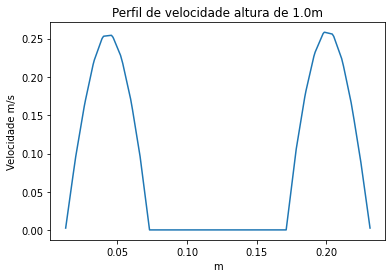
\includegraphics[width=\linewidth]{img/perfil_vel/liso/perfil_velocidade_liso_1000.png}
    	\end{subfigure}
    	\caption{Perfis de velocidade da geometria $A_1$ em 4 níveis distintos}
    	\label{fig:perfil_velocidade_liso}
\end{figure}
    
\begin{comment}
    Cada parâmetro calculado e seus respectivos níveis e lados são especificados na tabela \ref{tab:valor_parametro_A1}.

    \begin{table}[H]
        \centering
        \caption{valor do parâmetro de limpeza para cada nível na geometria $A_1$}
    	\begin{tabular}{ccc}
    		\hline
    		$q$ & $y_k$ & $\eta$ \\
    		\hline
    		E & 0.100 & 0.0744 \\
    		D  & 0.100 & 0.0747 \\
    		E & 0.300 & 0.0125 \\
    		D  & 0.300 & 0.0127 \\
    		E & 0.999 & 0.0274 \\
    		D  & 0.999 & 0.0277 \\
    		\hline
    	\end{tabular}
    	\label{tab:valor_parametro_A1}
    \end{table}
\end{comment}
    
Considerando agora a geometria $A_2$, de parede lisa e valor de \textit{standoff} de 50\%, o campo de velocidade na saída é mostrado na Fig. \ref{fig:perfil_velocidade_liso_saida_standoff_paraview}.
\begin{figure}[H]
        \centering
    	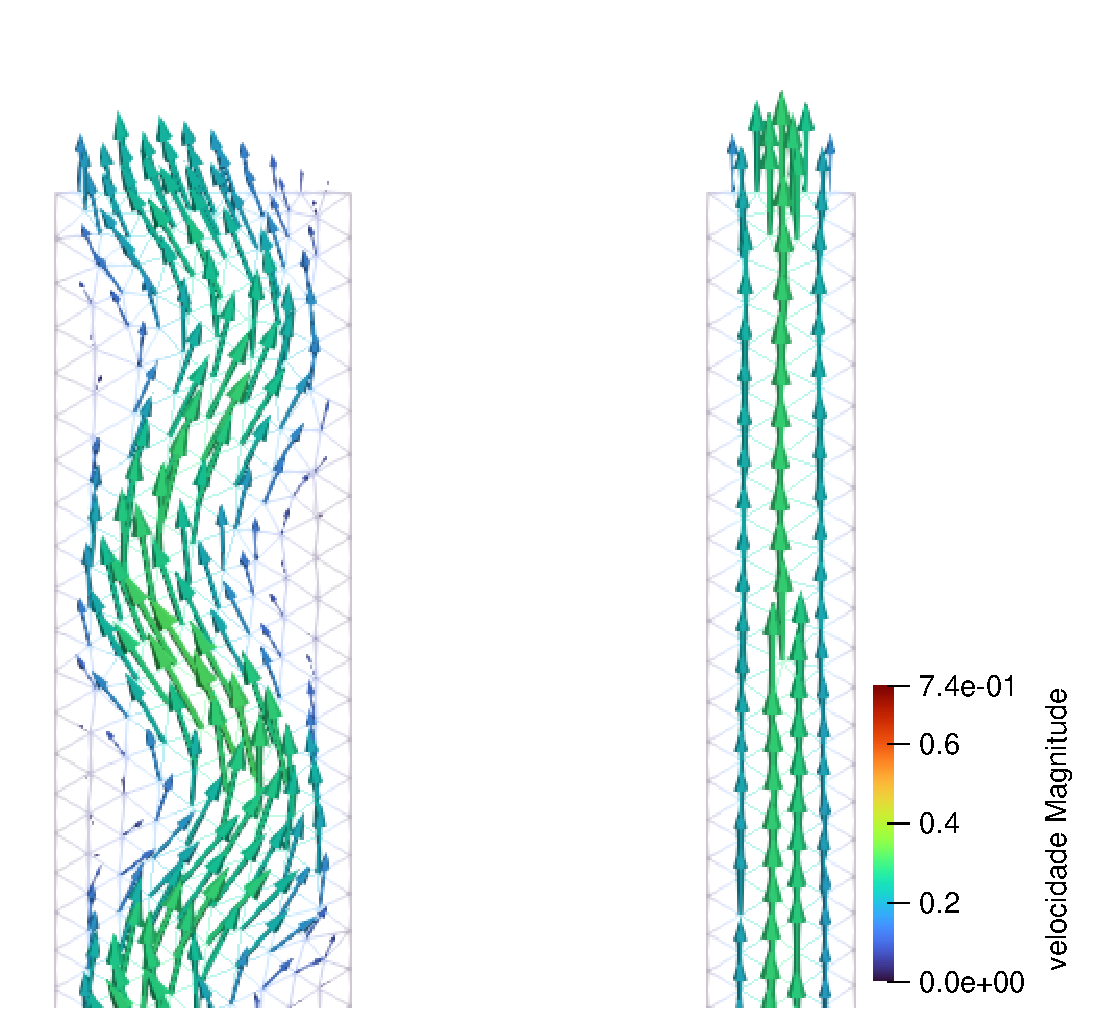
\includegraphics[scale=0.5]{img/perfil_vel/liso/perfil_de_vel_saida_standoff_paraview.eps}
    	\caption{Campo de velocidade na saída do espaço anular no tempo de 10s na geometria $A_2$. Fonte: autor}
    	\label{fig:perfil_velocidade_liso_saida_standoff_paraview}
\end{figure}
    
É evidente o efeito do standoff no escoamento, o fluxo teve um comportamento ondulatório. Na região da sapata, perto do fundo do poço Fig. \ref{fig:perfil_velocidade_liso_sapata_standoff_paraview_0_5s} é possível observar que do lado direito a velocidade teve um perfil mais regular que do lado esquerdo. 
     
\begin{figure}[H]
        \centering
        \begin{subfigure}[b]{0.42\linewidth}
    		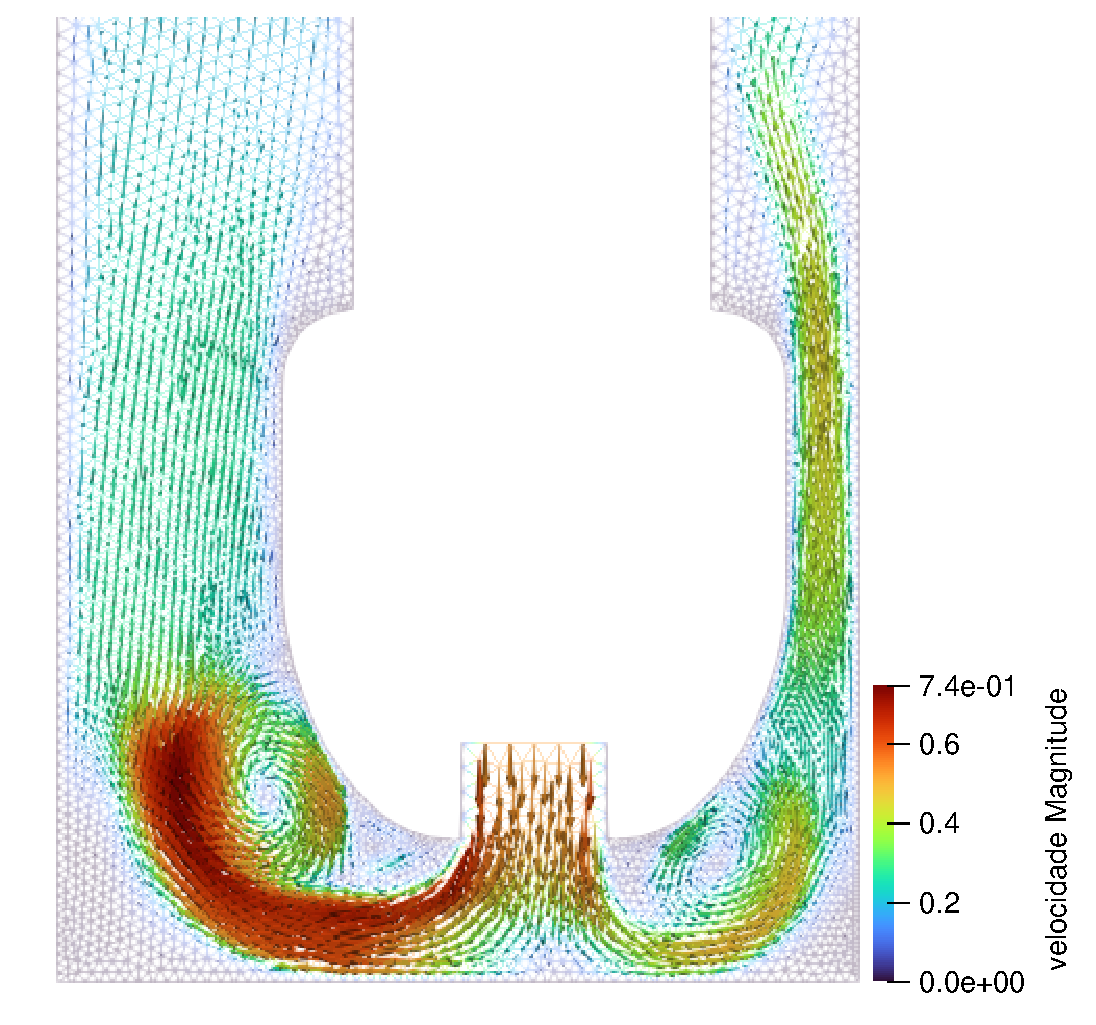
\includegraphics[width=\linewidth]{img/perfil_vel/liso/perfil_de_vel_sapata_standoff_paraview_0.5s.eps}
    	\end{subfigure}
    	\begin{subfigure}[b]{0.42\linewidth}
    		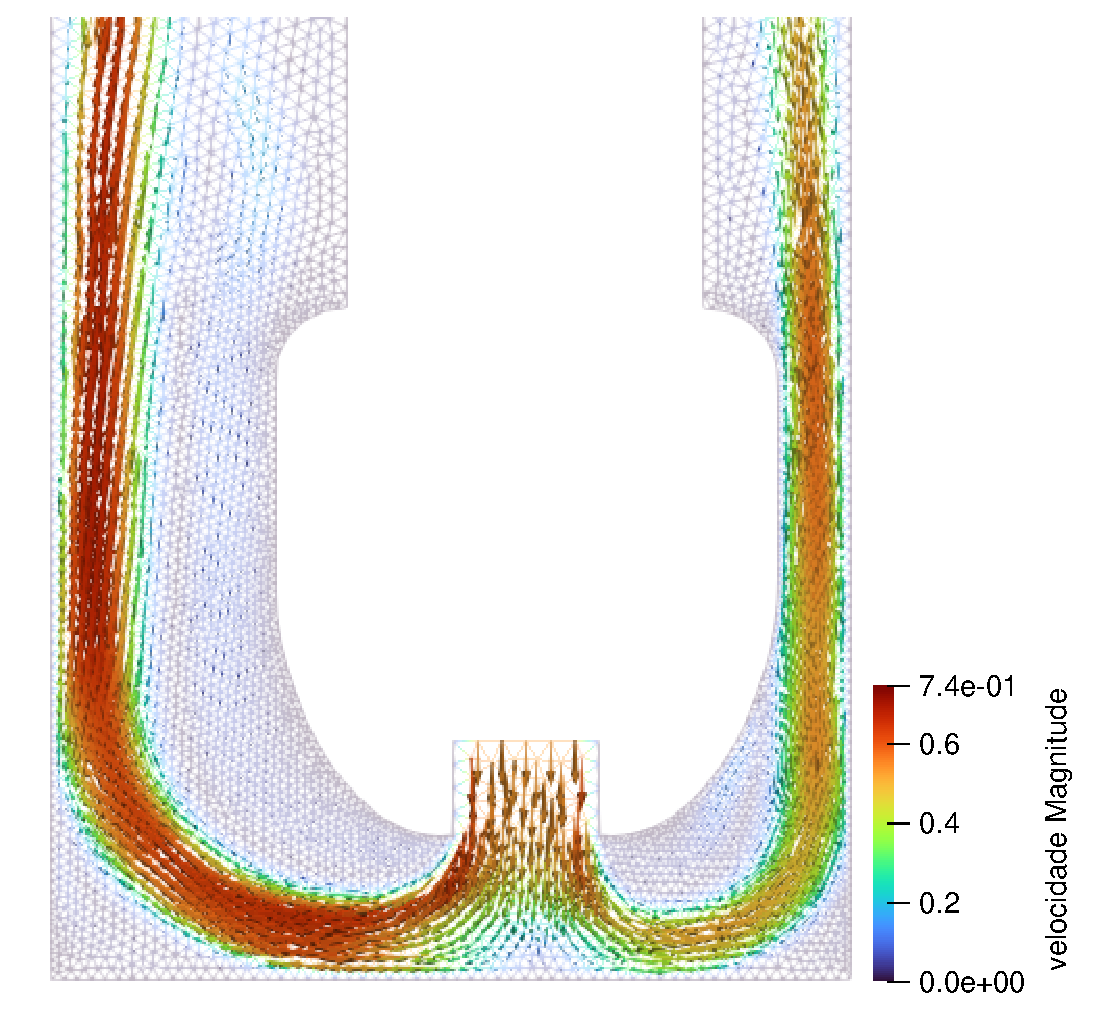
\includegraphics[width=\linewidth]{img/perfil_vel/liso/perfil_de_vel_sapata_standoff_paraview_10s.eps}
    	\end{subfigure}
    	\caption{Campo de velocidade na sapata no tempo de 0.5s e 10s na geometria $A_2$. Fonte: autor}
    	\label{fig:perfil_velocidade_liso_sapata_standoff_paraview_0_5s}
\end{figure}
    
Os perfis de velocidade para os 4 níveis selecionados na geometria onde não há nenhuma rugosidade na parede do poço e um valor de \textit{standoff} menor que 100\% podem ser visualizados na figura 
\begin{figure}[H]
    	\begin{subfigure}[b]{0.42\linewidth}
    		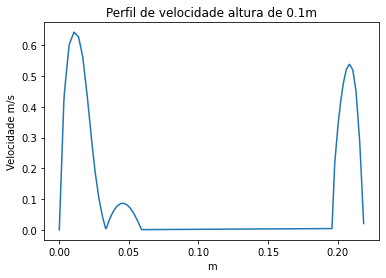
\includegraphics[width=\linewidth]{img/perfil_vel/liso/perfil_velocidade_liso_s_100.png}
    	\end{subfigure}
    	\begin{subfigure}[b]{0.42\linewidth}
    		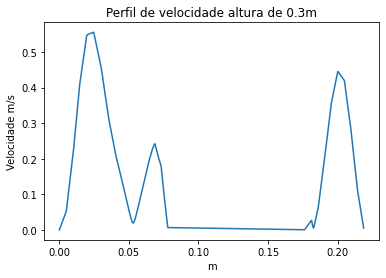
\includegraphics[width=\linewidth]{img/perfil_vel/liso/perfil_velocidade_liso_s_300.png}
    	\end{subfigure}
    	\\
    	\begin{subfigure}[b]{0.42\linewidth}
    		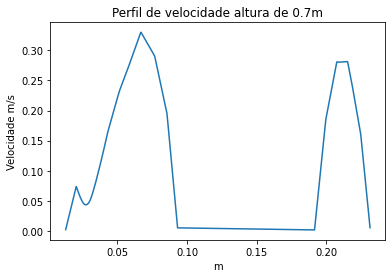
\includegraphics[width=\linewidth]{img/perfil_vel/liso/perfil_velocidade_liso_s_700.png}
    	\end{subfigure}
    	\begin{subfigure}[b]{0.42\linewidth}
    		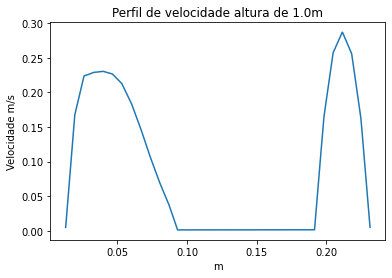
\includegraphics[width=\linewidth]{img/perfil_vel/liso/perfil_velocidade_liso_s_1000.png}
    	\end{subfigure}
    	\caption{Perfis de velocidade da geometria $A_2$ em 4 níveis distintos}
    	\label{fig:perfil_velocidade_liso_standoff}
\end{figure}
    
Recortes do campo de pressão das geometrias $A$ podem ser vistos na Fig. \ref{fig:cpressaoA1A2}
\begin{figure}[H]
        \centering
        \begin{subfigure}[b]{0.42\linewidth}
    		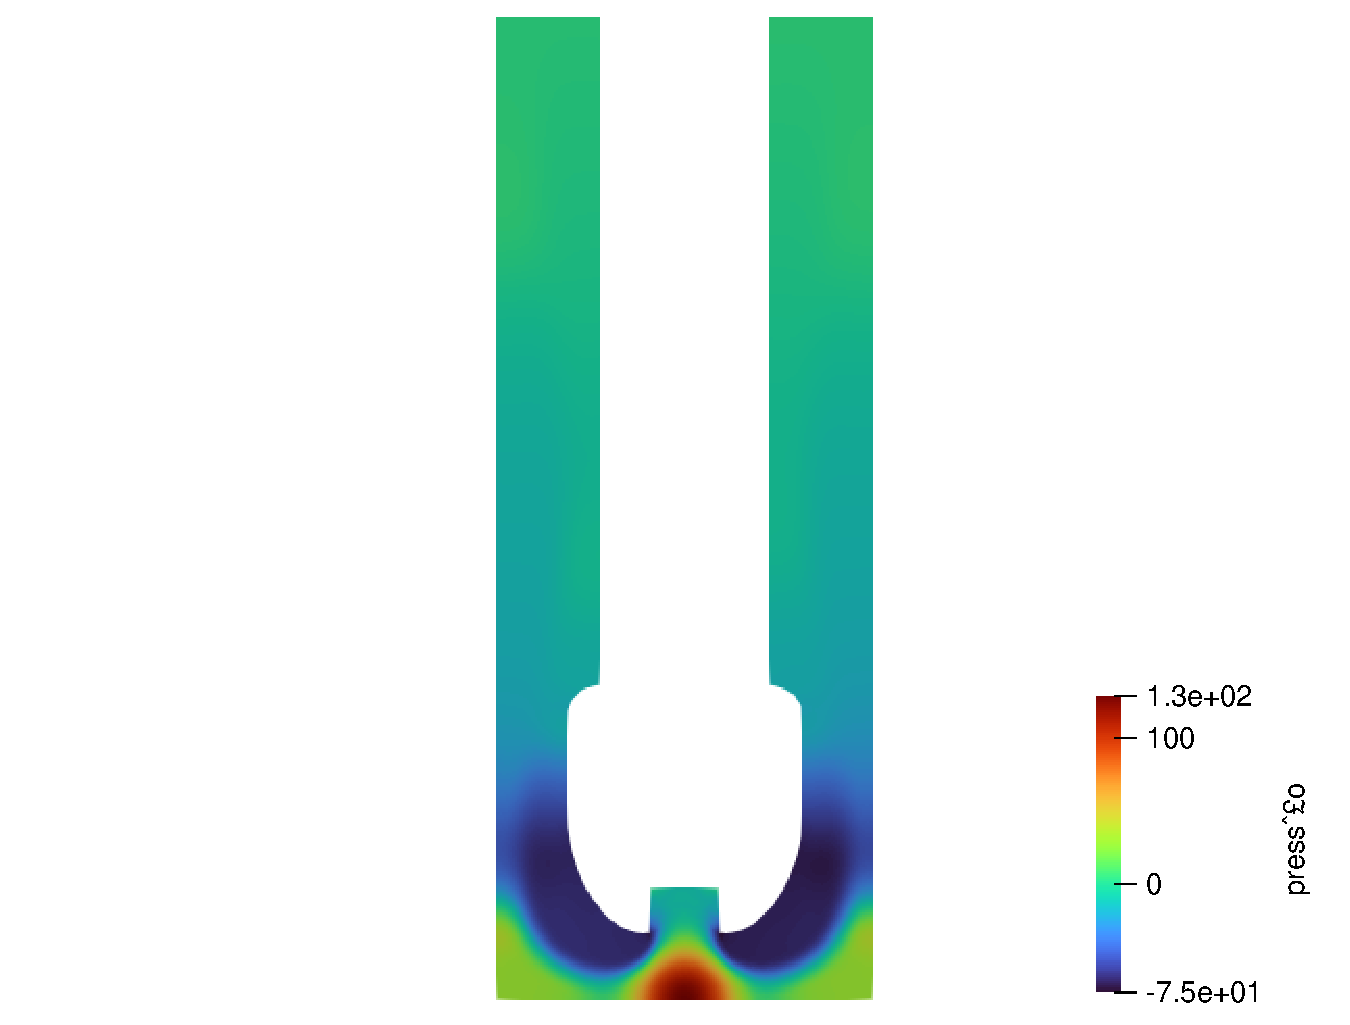
\includegraphics[width=\linewidth]{img/campo_press/liso/campo_de_pres_paraview.eps}
    	\end{subfigure}
    	\begin{subfigure}[b]{0.42\linewidth}
    		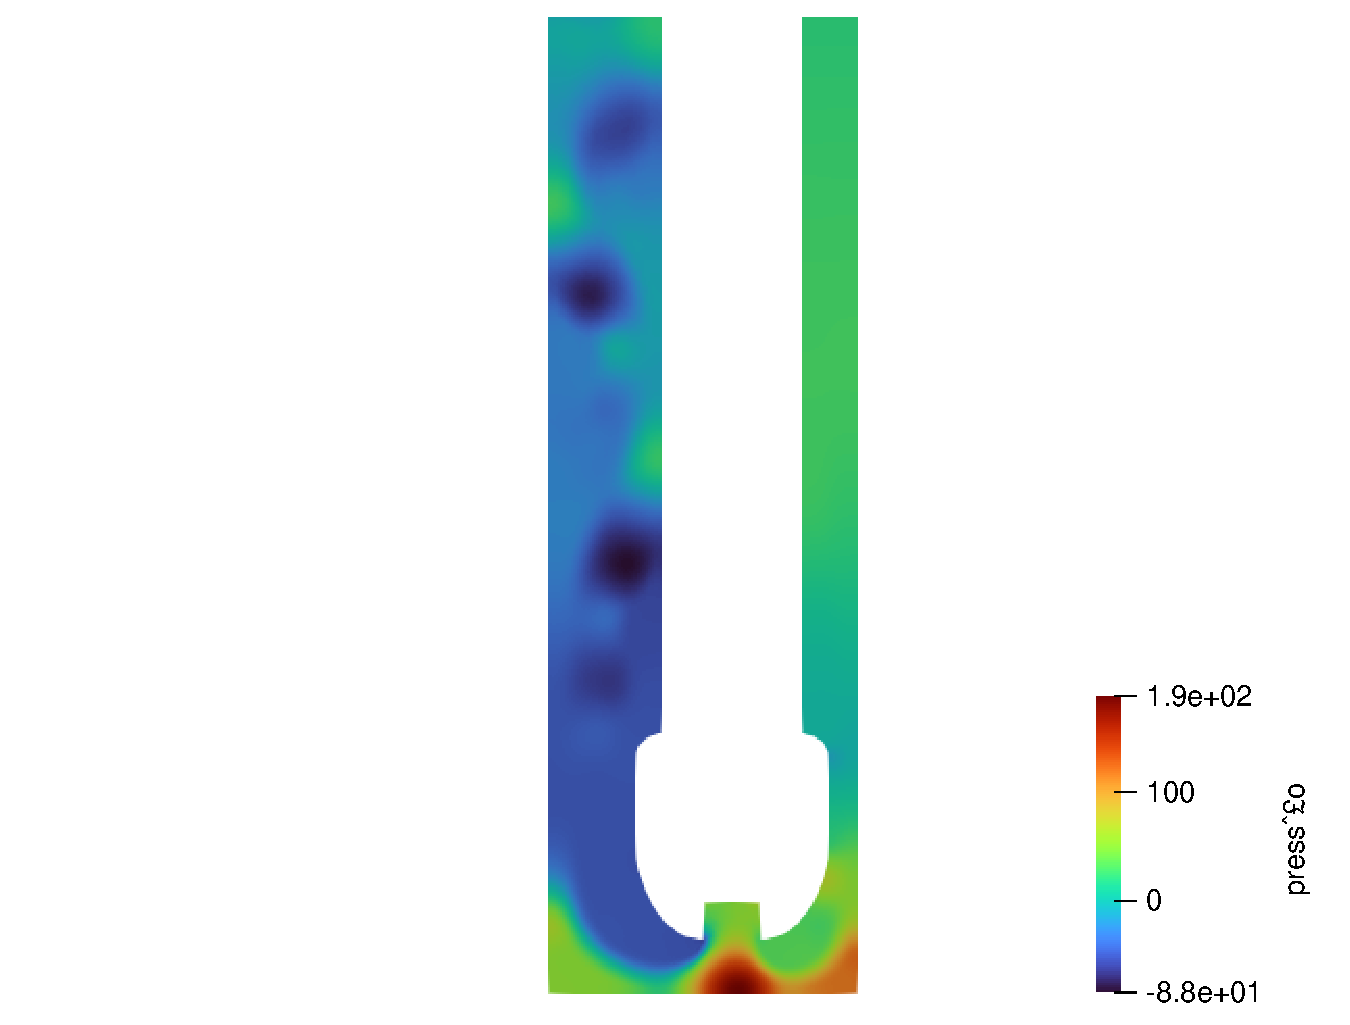
\includegraphics[width=\linewidth]{img/campo_press/liso/campo_de_pres_standoff_paraview.eps}
    	\end{subfigure}
    	\caption{Campo de pressão nas geometrias $A$. Fonte: autor}
    	\label{fig:cpressaoA1A2}
\end{figure}
    
\begin{comment}
    Cada parâmetro calculado e seus respectivos níveis e lados são especificados na tabela \ref{tab:valor_parametro_A2}.
    
    \begin{table}[H]
        \centering
        \caption{valor do parâmetro de limpeza para cada nível na geometria $A_2$}
    	\begin{tabular}{ccc}
    		\hline
    		$q$ & $y_k$ & $\eta$ \\
    		\hline
    		E & 0.100 & 0.0744 \\
    		D  & 0.100 & 0.0747 \\
    		E & 0.300 & 0.0125 \\
    		D  & 0.300 & 0.0127 \\
    		E & 0.999 & 0.0274 \\
    		D  & 0.999 & 0.0277 \\
    		\hline
    	\end{tabular}
    	\label{tab:valor_parametro_A2}
    \end{table}
\end{comment}


\subsubsection{Configurações com Erosões}
    
Para o caso das geometrias $B$, em que há um certo grau de erosão na parede da formação, o perfil de velocidade na saída do anular observado na Fig. \ref{fig:perfil_velocidade_rugoso_saida_paraview_10s} mostra um escoamento parabólico. O mesmo comportamento foi visto nas geometrias $A$. Logo, a erosão não causou interferências.
\begin{figure}[H]
        \centering
    	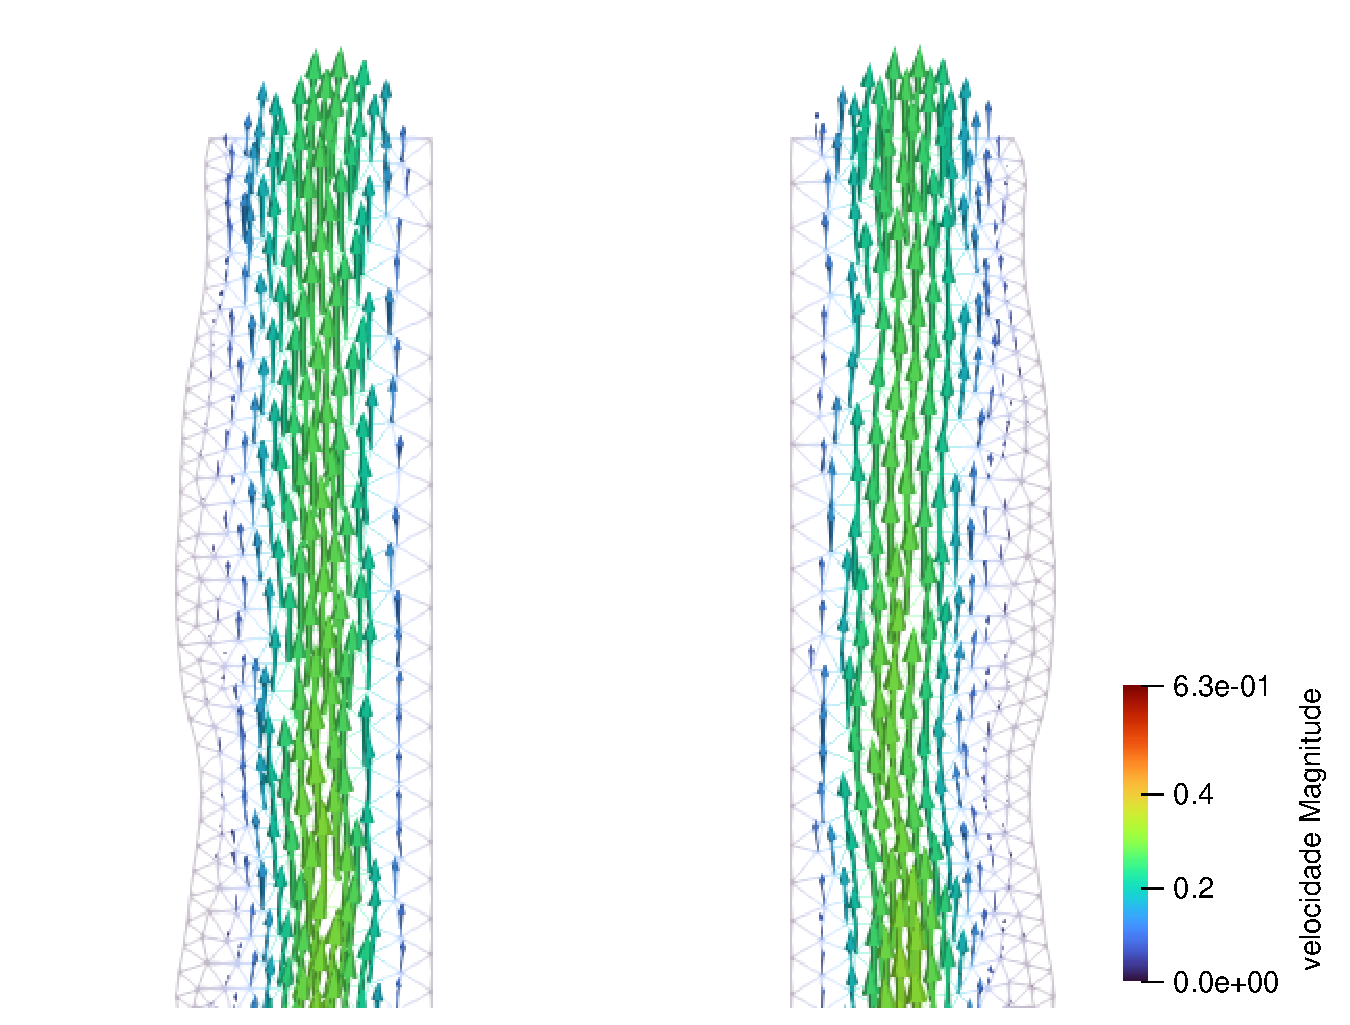
\includegraphics[scale=0.5]{img/perfil_vel/rugoso/perfil_de_vel_saida_paraview.eps}
    	\caption{Campo de velocidade na saída do espaço anular no tempo de 10s na geometria $B_1$. Fonte: autor}
    	\label{fig:perfil_velocidade_rugoso_saida_paraview_10s}
\end{figure}
    
A Fig. \ref{fig:perfil_velocidade_rugoso_sapata_paraview_0.5s} mostra o comportamento do fluido na sapata no tempo de $0.5s$ e $10s$ evidenciando o efeito da erosão se comparado a Fig. \ref{fig:perfil_velocidade_liso_sapata_paraview_0_5s} pode-se observar que o comportamento do fluido foi simétrico como na geometria $A_1$ e concluir que o efeito da erosão nesse caso não teve impacto expressivo
    
    \begin{figure}[H]
        \centering
        \begin{subfigure}[b]{0.42\linewidth}
            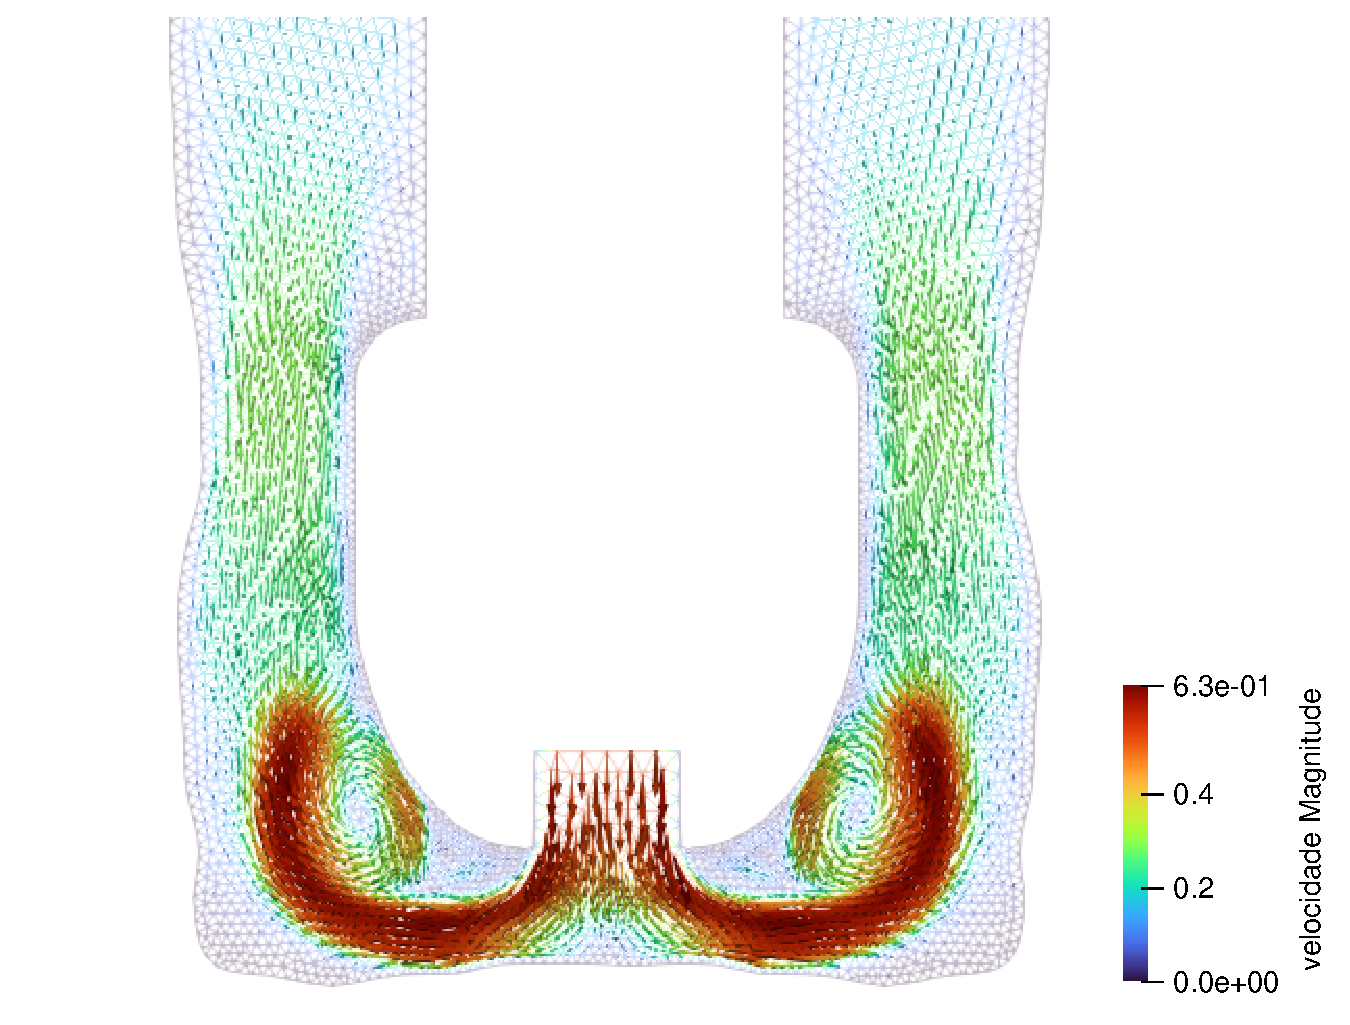
\includegraphics[width=\linewidth]{img/perfil_vel/rugoso/perfil_de_vel_sapata_paraview_0.5s.eps}
        \end{subfigure}
        \begin{subfigure}[b]{0.42\linewidth}
            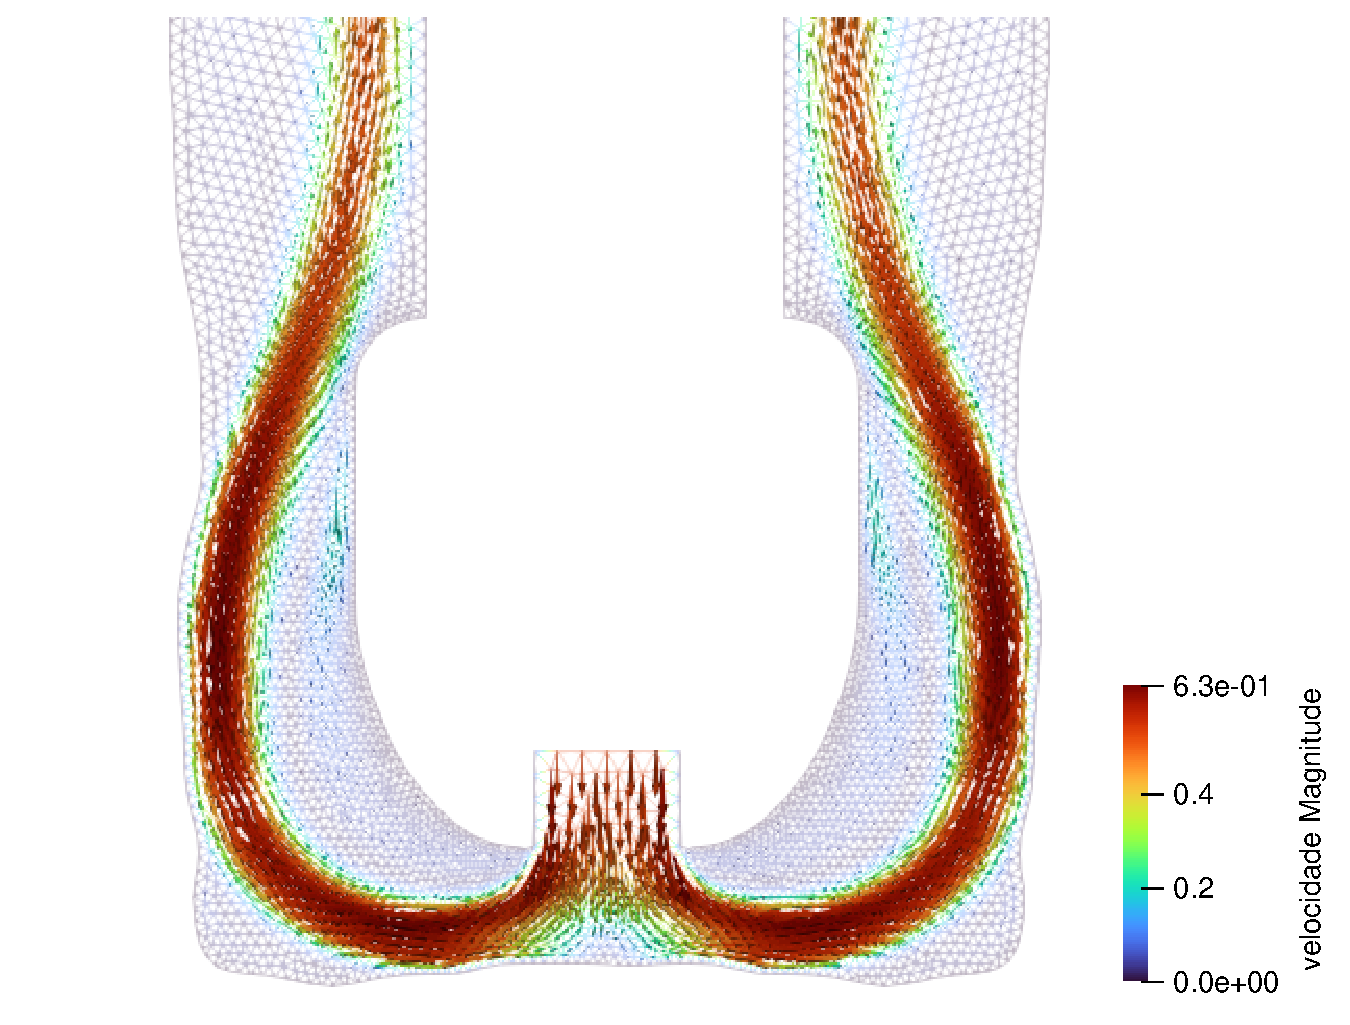
\includegraphics[width=\linewidth]{img/perfil_vel/rugoso/perfil_de_vel_sapata_paraview_10s.eps}
        \end{subfigure}
    	
    	\caption{Campo de velocidade na sapata no tempo de 0.5s e 10s na geometria $B_1$. Fonte: autor}
    	\label{fig:perfil_velocidade_rugoso_sapata_paraview_0.5s}
    \end{figure}
    
Os perfis de velocidade para os 4 níveis selecionados na geometria onde há rugosidade na parede do poço e um valor de \textit{standoff} igual a 100\% ($B_1$) podem ser visualizados na figura \ref{fig:perfil_velocidade_rugosa}.
    \begin{figure}[H]
        \centering
    	\begin{subfigure}[b]{0.42\linewidth}
    		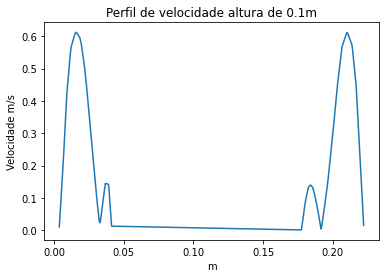
\includegraphics[width=\linewidth]{img/perfil_vel/rugoso/perfil_velocidade_rugoso_100.png}
    	\end{subfigure}
    	\begin{subfigure}[b]{0.42\linewidth}
    		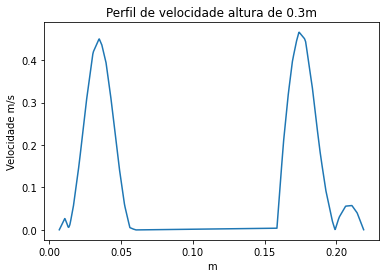
\includegraphics[width=\linewidth]{img/perfil_vel/rugoso/perfil_velocidade_rugoso_300.png}
    	\end{subfigure}
    	\\
    	\begin{subfigure}[b]{0.42\linewidth}
    		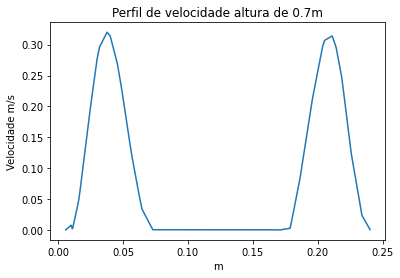
\includegraphics[width=\linewidth]{img/perfil_vel/rugoso/perfil_velocidade_rugoso_700.png}
    	\end{subfigure}
    	\begin{subfigure}[b]{0.42\linewidth}
    		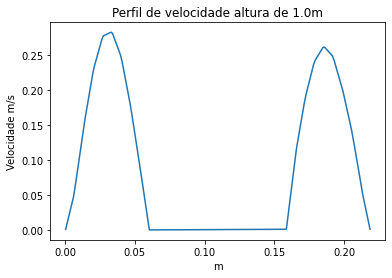
\includegraphics[width=\linewidth]{img/perfil_vel/rugoso/perfil_velocidade_rugoso_1000.png}
    	\end{subfigure}
    	\caption{Perfis de velocidade da geometria $B_1$ em 4 níveis distintos}
    	\label{fig:perfil_velocidade_rugosa}
    \end{figure}
    
\begin{comment}
    Cada parâmetro calculado e seus respectivos níveis e lados são especificados na tabela \ref{tab:valor_parametro_B1}.
    
    \begin{table}[H]
        \centering
        \caption{valor do parâmetro de limpeza para cada nível na geometria $B_1$}
    	\begin{tabular}{ccc}
    		\hline
    		$q$ & $y_k$ & $\eta$ \\
    		\hline
    		E & 0.100 & 0.0744 \\
    		D  & 0.100 & 0.0747 \\
    		E & 0.300 & 0.0125 \\
    		D  & 0.300 & 0.0127 \\
    		E & 0.999 & 0.0274 \\
    		D  & 0.999 & 0.0277 \\
    		\hline
    	\end{tabular}
    	\label{tab:valor_parametro_B1}
    \end{table}
\end{comment}
   
Para o caso da geometria $B_2$, onde a taxa de \textit{standoff} é de 50\%, o perfil de velocidade na saída do anular observado na Fig. \ref{fig:perfil_velocidade_rugoso_saida_paraview_10s} mostra um escoamento parabólico, esse mesmo comportamento foi visto nas geometrias $A$, portanto, a erosão não causou interferência nesse sentido, porém a erosão causou um efeito de irregularidade no escoamento com pequenas zonas de recirculação.
    
\begin{figure}[H]
        \centering
    	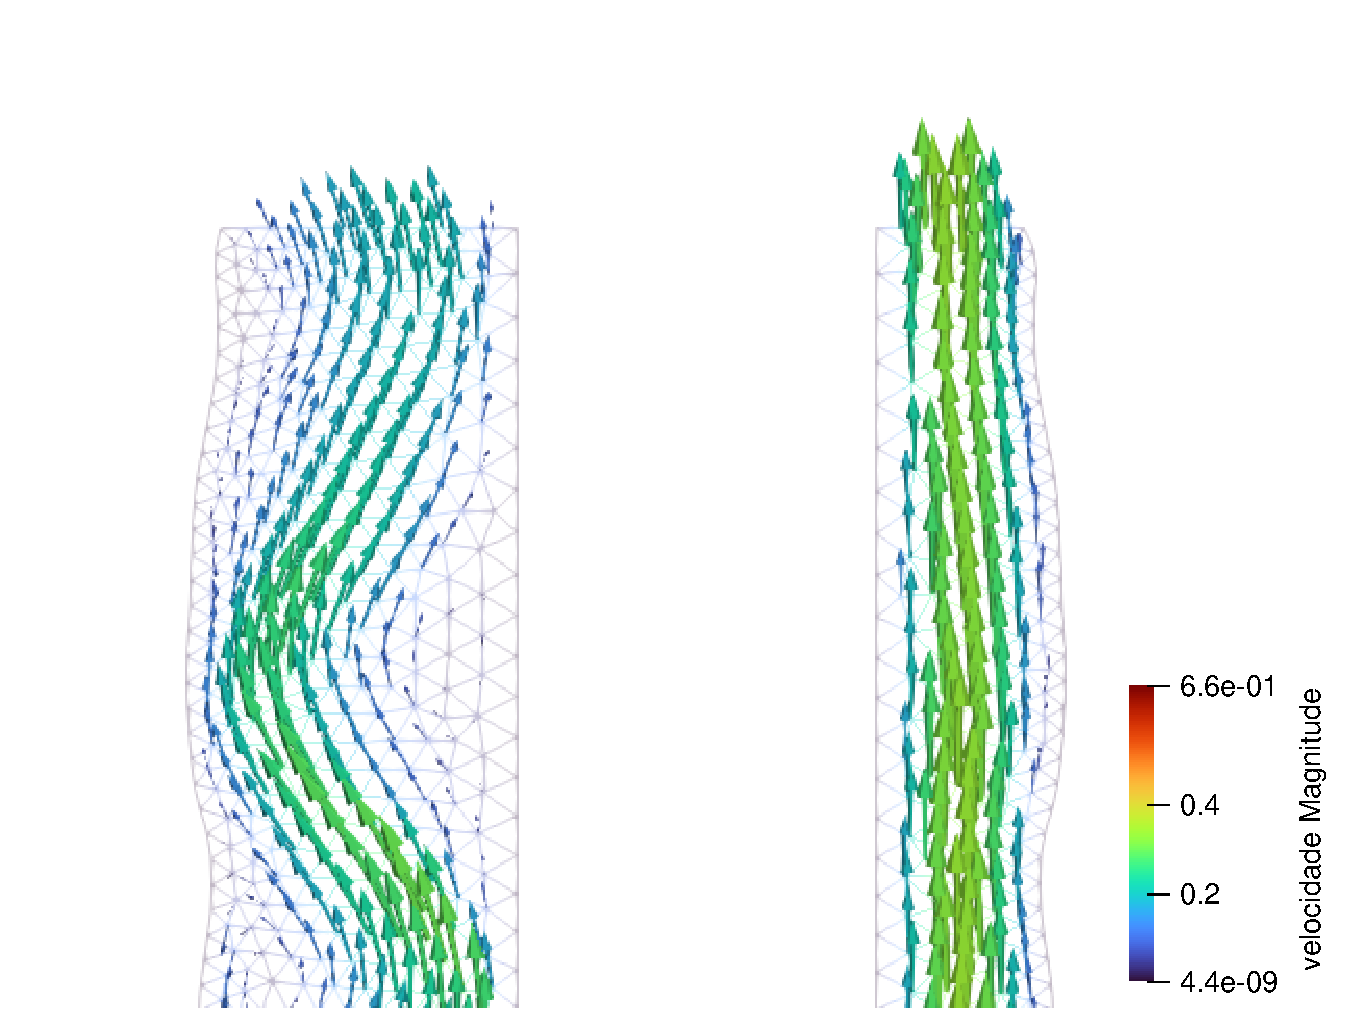
\includegraphics[scale=0.5]{img/perfil_vel/rugoso/perfil_de_vel_saida_standoff_paraview.eps}
    	\caption{Campo de velocidade na saída do espaço anular no tempo de 10s na geometria $B_2$. Fonte: autor}
    	\label{fig:perfil_velocidade_rugoso_saida_paraview_10s}
\end{figure}
    
A Fig. \ref{fig:perfil_velocidade_rugoso_sapata_standoff_paraview_0.5s} mostra o comportamento do fluido na sapata nos tempos de $0.5s$ e $10s$ evidenciando o efeito da erosão se comparado a Fig. \ref{fig:perfil_velocidade_liso_sapata_standoff_paraview_0_5s} pode-se observar que o comportamento do fluido não foi simétrico como na geometria $A_2$
    \begin{figure}[H]
        \centering
        \begin{subfigure}[b]{0.42\linewidth}
            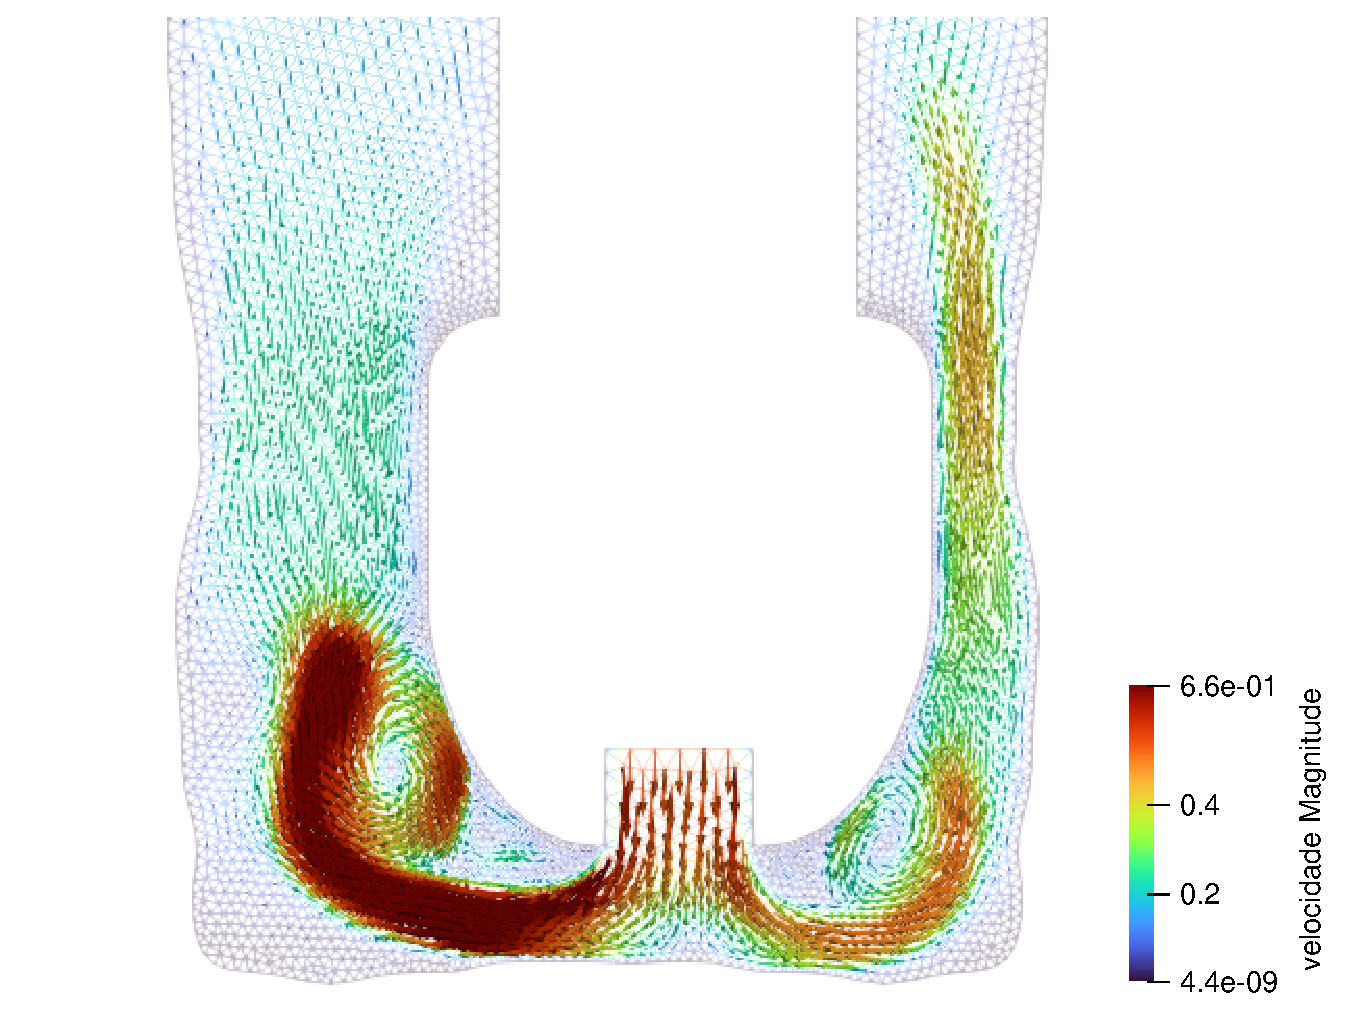
\includegraphics[width=\linewidth]{img/perfil_vel/rugoso/perfil_de_vel_sapata_standoff_paraview_0_5s.eps}
        \end{subfigure}
        \begin{subfigure}[b]{0.42\linewidth}
            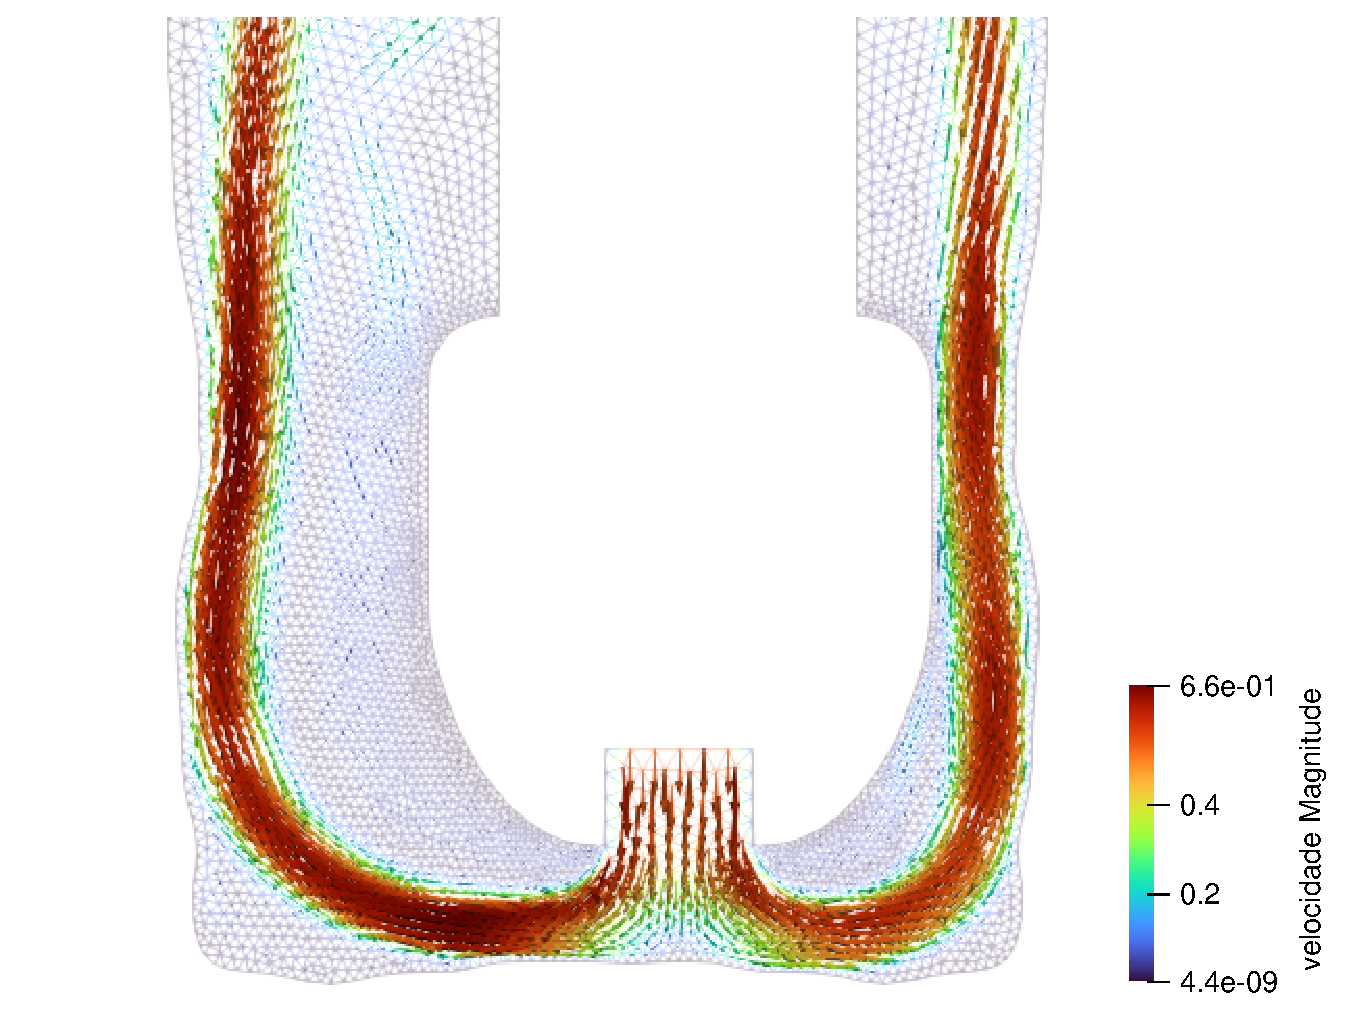
\includegraphics[width=\linewidth]{img/perfil_vel/rugoso/perfil_de_vel_sapata_standoff_paraview_10s.eps}
        \end{subfigure}
    	
    	\caption{Campo de velocidade na sapata no tempo de 0.5s e $10s$ na geometria $B_2$. Fonte: autor}
    	\label{fig:perfil_velocidade_rugoso_sapata_standoff_paraview_0.5s}
    \end{figure}
    
Os perfis de velocidade para os 4 níveis selecionados na geometria onde há rugosidade na parede do poço e um valor de \textit{standoff} menor que 100\% $B_2$ podem ser visualizado na figura \ref{fig:perfil_velocidade_rugosa_standoff}.
    \begin{figure}[H]
    	\begin{subfigure}[b]{0.42\linewidth}
    		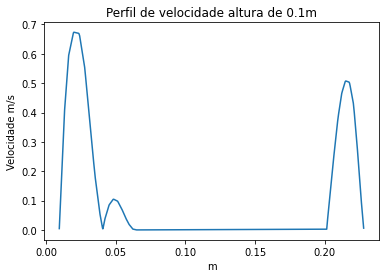
\includegraphics[width=\linewidth]{img/perfil_vel/rugoso/perfil_velocidade_rugoso_s_100.png}
    	\end{subfigure}
    	\begin{subfigure}[b]{0.42\linewidth}
    		\includegraphics[width=\linewidth]{img/perfil_vel/rugoso/perfil_velocidade_rugoso_s_300.png}
    	\end{subfigure}
    	\\
    	\begin{subfigure}[b]{0.42\linewidth}
    		\includegraphics[width=\linewidth]{img/perfil_vel/rugoso/perfil_velocidade_rugoso_s_700.png}
    	\end{subfigure}
    	\begin{subfigure}[b]{0.42\linewidth}
    		\includegraphics[width=\linewidth]{img/perfil_vel/rugoso/perfil_velocidade_rugoso_s_1000.png}
    	\end{subfigure}
    	\caption{Perfis de velocidade da geometria $B_2$ para 4 níveis distintos}
    	\label{fig:perfil_velocidade_rugosa_standoff}
    \end{figure}
    
Recortes do campo de pressão das geometrias $B$ podem ser vistos na Fig. \ref{fig:cpressaoB1B2}.
\begin{figure}[H]
        \centering
        \begin{subfigure}[b]{0.42\linewidth}
    		\includegraphics[width=\linewidth]{img/campo_press/rugoso/campo_de_pres_paraview.eps}
    	\end{subfigure}
    	\begin{subfigure}[b]{0.42\linewidth}
    		\includegraphics[width=\linewidth]{img/campo_press/rugoso/campo_de_pres_standoff_paraview.eps}
    	\end{subfigure}
    	\caption{Campo de pressão nas geometrias $B$. Fonte: autor}
    	\label{fig:cpressaoB1B2}
\end{figure}

\begin{comment}
Cada parâmetro calculado e seus respectivos níveis e lados são especificados na tabela \ref{tab:valor_parametro_B2}.
    
    \begin{table}[H]
        \centering
        \caption{valor do parâmetro de limpeza para cada nível na geometria $B_2$}
    	\begin{tabular}{ccc}
    		\hline
    		$q$ & $y_k$ & $\eta$ \\
    		\hline
    		E & 0.100 & 0.0744 \\
    		D  & 0.100 & 0.0747 \\
    		E & 0.300 & 0.0125 \\
    		D  & 0.300 & 0.0127 \\
    		E & 0.999 & 0.0274 \\
    		D  & 0.999 & 0.0277 \\
    		\hline
    	\end{tabular}
    	\label{tab:valor_parametro_B2}
    \end{table}
    
    A tabela \ref{tab:tabela_resultado_geral} contem os resultados de forma geral.
    
    \begin{table}[H]
        \centering
        \caption{valor do parâmetro de limpeza para cada nível na geometria do lado esquerdo $B_2$}
    	\begin{tabular}{cccccc}
    		\hline
    		$Q_l^A$ & $Q_l^B$ & $h$ & $\eta_a$ & $\eta_b$ & $\eta$ \\
    		\hline
    		50.92 & 33.00 & 0.1 & 0.0745 & 0.5944 & 7.97 \\
    		48.51  & 47.34 & 0.3 & 0.0126 & 0.0289 & 2.29 \\
    		43.68 & 40.55 & 0.7 & 0.0283 & 0.0377 & 1.33 \\
    		43.67 & 40.09 & 1 & 0.0276 & 0.0292 & 1.06 \\
    		\hline
    	\end{tabular}
    	\label{tab:tabela_resultado_geral}
    \end{table}
\end{comment}

\subsubsection{Análise de eficiência de varrido}

A fim de comparar a eficiência de varrido, as tabelas \ref{tab:tabela_resultado_geralA1B1E}, \ref{tab:tabela_resultado_geralA1B1D}, \ref{tab:tabela_resultado_geralA2B2E} e  \ref{tab:tabela_resultado_geralA2B2D} abaixo, descrevem as vazões $Q$ em cada geometria e o parâmetro $\eta$ dos respectivos lados do espaço anular. É descrito também os valores da vazão $Q$ e do $\eta$ no espaço delimitado em $90\%$ e no espaço total. 
    
O parâmetro de eficiência de varrido $\eta$ do lado esquerdo do espaço anular levando em consideração as geometrias $A_1$ e $B_1$ ficou em torno de 0.9 a exceção do valor delimitado em 90\% perto do fundo do poço em $0.1m$ onde foi de 0.53, tabela \ref{tab:tabela_resultado_geralA1B1E}, isto é, há uma eficiência, no caso em que há erosão, de 90\% do caso ideal (liso) em níveis acima de $0.3m$, em $0.1m$ a erosão causou uma ineficiência de aproximadamente 50\% em relação ao caso ideal (liso) se levarmos em consideração o espaço delimitado em 90\%. Esta análise é análoga ao lado direito, tabela \ref{tab:tabela_resultado_geralA1B1D} das mesmas geometrias por se tratar de um caso de \textit{standoff} de 100\%.  
    
    \begin{table}[H]
        \centering
        \caption{Valor do parâmetro $\eta$ para cada nível das geometrias $A_1$ e $B1$ do lado esquerdo}
    	\begin{tabular}{cccccccc}
    		\hline
    		$k$ & $y_k$ & $Q_A^E$ & $Q_{A,90}^E$ & $Q_B^E$ & $Q_{B,90}^E$ & $\eta_{90}^E$ & $\eta^E$ \\
    		\hline
    		1 & 0.1 & 45.18 & 41.42 & 41.64 & 22.06 & 53.27\% & 92.17\% \\
    		2 & 0.3 & 45.28 & 45.89 & 41.42 & 42.78 & 93.23\% & 91.46\% \\
    		3 & 0.7 & 44.92 & 43.68 & 41.22 & 40.00 & 91.57\% & 91.77\% \\
    		4 & 1.0 & 44.93 & 43.74 & 41.22 & 40.00 & 91.44\% & 91.74\% \\
    		\hline
    	\end{tabular}
    	\label{tab:tabela_resultado_geralA1B1E}
    \end{table}
    
    \begin{table}[H]
        \centering
        \caption{Valor do parâmetro $\eta$ para cada nível das geometrias $A_1$ e $B1$ do lado direito}
    	\begin{tabular}{cccccccc}
    		\hline
    		$k$ & $y_k$ & $Q_A^D$ & $Q_{A,90}^D$ & $Q_B^D$ & $Q_{B,90}^D$ & $\eta_{90}^D$ & $\eta^D$ \\
    		\hline
    		1 & 0.1 & 46.14 & 42.24 & 41.63 & 17.17 & 40.64\% & 90.21\% \\
    		2 & 0.3 & 46.10 & 46.69 & 41.54 & 43.22 & 92.57\% & 90.12\% \\
    		3 & 0.7 & 45.63 & 44.42 & 41.08 & 39.68 & 89.34\% & 90.03\% \\
    		4 & 1.0 & 45.72 & 44.52 & 41.08 & 39.68 & 89.12\% & 89.85\% \\
    		\hline
    	\end{tabular}
    	\label{tab:tabela_resultado_geralA1B1D}
    \end{table}
    
O parâmetro de eficiência de varrido $\eta$ do lado esquerdo do espaço anular levando em consideração as geometrias $A_2$ e $B_2$ ficou em torno de 0.6 a 0.8 a exceção do valor perto ao fundo do poço em $0.1m$ onde foi de 0.37, tabela \ref{tab:tabela_resultado_geralA1B1E}, isto é, há uma eficiência no caso da erosão de 90\% do caso ideal (liso) em níveis acima de $0.3m$, em $0.1m$ a erosão causou uma ineficiência de aproximadamente 37\% em relação ao caso ideal (liso), considerando apenas o espaço delimitado em 90\%. 
    
Como o valor de \textit{standoff} não é 100\% aqui, então há uma grande diferença dos valores de $\eta$ no espaço anular de menor distância, visto que o escoamento possui menos espaço para percorrer, ele preenche todo o espaço direito, e a eficiência aumenta, o inverso acontece no lado esquerdo, onde os valores foram menos que 0.9 no caso simétrico. No lado direito a eficiência de varrido teve uma melhoria quando a parede foi erodida com um valor de $115\%$ do caso ideal (liso).
    
    \begin{table}[H]
        \centering
        \caption{Valor do parâmetro $\eta$ para cada nível das geometrias $A_2$ e $B2$ do lado esquerdo}
    	\begin{tabular}{cccccccc}
    		\hline
    		$k$ & $y_k$ & $Q_A^E$ & $Q_{A,90}^E$ & $Q_B^E$ & $Q_{B,90}^E$ & $\eta_{90}^E$ & $\eta^E$ \\
    		\hline
    		1 & 0.1 & 55.58 & 44.20 & 42.11 & 16.72 & 37.82\% & 75.77\% \\
    		2 & 0.3 & 56.63 & 54.88 & 43.35 & 42.99 & 78.34\% & 76.55\% \\
    		3 & 0.7 & 54.83 & 56.20 & 42.17 & 35.74 & 63.58\% & 76.91\% \\
    		4 & 1.0 & 55.74 & 51.93 & 42.08 & 41.05 & 79.05\% & 75.49\% \\
    		\hline
    	\end{tabular}
    	\label{tab:tabela_resultado_geralA2B2E}
    \end{table}
    
    \begin{table}[H]
        \centering
        \caption{Valor do parâmetro $\eta$ para cada nível das geometrias $A_2$ e $B2$ do lado direito}
    	\begin{tabular}{cccccccc}
    		\hline
    		$k$ & $y_k$ & $Q_A^D$ & $Q_{A,90}^D$ & $Q_B^D$ & $Q_{B,90}^D$ & $\eta_{90}^D$ & $\eta^D$ \\
    		\hline
    		1 & 0.1 & 34.74 & 33.24 & 40.95 & 25.33 & 76.20\% & 117.86\% \\
    		2 & 0.3 & 35.37 & 34.56 & 40.78 & 29.86 & 86.40\% & 115.27\% \\
    		3 & 0.7 & 33.95 & 32.92 & 40.58 & 35.48 & 107.78\% & 119.53\% \\
    		4 & 1.0 & 34.32 & 33.27 & 39.06 & 37.59 & 113.00\% & 113.82\% \\
    		\hline
    	\end{tabular}
    	\label{tab:tabela_resultado_geralA2B2D}
    \end{table}
    
Os gráficos \ref{fig:eta_simetrico} e \ref{fig:eta_standoff} ilustra esse comportamento analisado nas 4 tabelas.
    
    \begin{figure}[H]
        \centering
        \begin{subfigure}[b]{0.42\linewidth}
    		\includegraphics[width=\linewidth]{img/eta/eta_esquerdo_simetrico.png}
    	\end{subfigure}
    	\begin{subfigure}[b]{0.42\linewidth}
    		\includegraphics[width=\linewidth]{img/eta/eta_direito_simetrico.png}
    	\end{subfigure}
    	\caption{Valores de $\eta$ para as geometrias com o valor de \textit{standoff} 100\% ($A_1$ e $B_1$). Fonte: autor}
    	\label{fig:eta_simetrico}
    \end{figure}
    
    \begin{figure}[H]
        \centering
        \begin{subfigure}[b]{0.42\linewidth}
    		\includegraphics[width=\linewidth]{img/eta/eta_esquerdo_standoff.png}
    	\end{subfigure}
    	\begin{subfigure}[b]{0.42\linewidth}
    		\includegraphics[width=\linewidth]{img/eta/eta_direito_standoff.png}
    	\end{subfigure}
    	\caption{Valores de $\eta$ para as geometrias com o valor de \textit{standoff} 50\%  ($A_2$ e $B_2$). Fonte: autor}
    	\label{fig:eta_standoff}
    \end{figure}

\section{CONCLUSÃO}

Este trabalho apresentou um estudo sobre o comportamento de colchões lavadores a base de óleo vegetal. O escoamento desse tipo de fluido ocorre durante a fase de pré-cimentação de poços de petróleo. Simulamos a dinâmica em diferentes tipos de geometrias de admitindo erosões e excentricidade do revestimento (\textit{standoff}). A fim de estudar a eficiência de varrido, um parâmetro tomando como referência a configuração de poço ideal, sem rugosidade nas paredes da formação. 

%Os códigos foram implementados em python e as simulações numéricas realizadas foi utilizando a biblioteca de domínio público FEniCS. O método dos elementos finitos foi aplicado para resolver as equações de Navier-Stokes. Para solucionar os sistemas lineares decorrente da discretização do problema foi utilizado o Método do
%Gradiente Biconjugado Estabilizado (bicgstab) para o cálculo da tentativa de velocidade e pressão com o precondicionador (HYPRE\_AMG), e para a correção da velocidade foi utilizado o método cg com o precondicionador sor. Os desenhos do revestimento para construção das malhas foram feitos no AutoCad e as malhas geradas no Gmsh. Os resultados obtidos mostraram que a excentricidade causa irregularidades no escoamento do fluido além de tornar a eficiência de varrido no espaço anular de maior largura mais baixo que no espaço anular de menor largura. A erosão torna o escoamento irregular em alguns casos, e perto do fundo do poço, o efeito da rugosidade é mais evidente, causando uma ineficiência de aproximadamente 50\%. 

Algumas limitações que tornam as simulações um pouco aquém da realidade tiveram de ser tratadas, tais como o nível do refinamento de malha, cuja captura dos perfis de velocidade não tiveram suavidade suficiente. Em segundo lugar, vale dizer que fluidos newtonianos não representam com exatidão o escoamento de colchões lavadores, visto que, em geral, modelos não-newtonianos, tais como o de Herschel-Bulkley são comumente utilizados. 

A extensão de estudo do poço foi limitada a $1m$, além de considerarmos a hipótese de poço raso, onde variações da força gravitacional praticamente são desprezíveis. %O tempo de execução das simulações foi de apenas $10s$, o que pode ter sido pouco para que o escoamento se desenvolvesse. Entretanto, esse tempo não pode ser maior devido ao número de iterações que precisaria ser maior e consequentemente maior o tempo de execução ou poder de processamento. 
Outro fator a ser levado em consideração é que em configurações com \emph{standoff}, geometrias bidimensionais são limitadas ao plano de simetria da configuração. Em ambas as configurações, tanto concêntricas como excêntricas, as ``vazões'' calculadas também perdem o seu sentido original, passando a medir uma espécie de ``fluxo planar''. 

Apesar disso, este trabalho destaca o potencial do método dos elementos finitos para tratar de problemas relacionados à cimentação primária de poços de petróleo, bem como desafios relacionados associados à engenharia de poços.

Como trabalhos futuros, listamos algumas sugestões:
\begin{itemize}
    \item implementar modelo não-newtoniano que represente melhor o tipo de escoamento de colchões lavadores a base de óleo vegetal;
    \item criar geometrias tridimensionais para melhor representar a formação rochosa, a topologia das erosões, a frente de propagação do fluido, interfaces e vazões reais; 
    \item melhorar a definição do coeficiente que mede a eficiência de varrido para levar em consideração outras características essenciais do escoamento; 
    \item realizar simulações de fluidos com outras propriedades.
\end{itemize}

%% --- ELEMENTOS PÓS-TEXTUAIS 

\renewcommand{\refname}{\flushleft REFERÊNCIAS} %Centraliza nome Referencias%
\addcontentsline{toc}{section}{REFERÊNCIAS} %adiciona referencias ao sumario
\begin{thebibliography}{99}
% As referências devem seguir o padrão da ABNT.

%para livro%
%SOBRENOME, Nome; SOBRENOME, Nome; SOBRENOME, Nome. Título: subtítulo (se houver). Edição (se houver). Local: Editora, ano de publicação.

\bibitem{KOEHLER}KOEHLER, Leonardo Pereira. {\bf Projeto de revestimento de popos e suas especificações.} 2018.

\bibitem{Elias} ELIAS, R. N. {\bf Estrutura de dados por arestas para a simulação paralela de escoamentos incompressíveis pelo método estabilizado de elementos finitos.} UFRJ, 2007.

\bibitem{Erik} NELSON, Erik B.; GUILLOT, Dominique. {\bf Well Cementing}. 2ª Edition. 

\bibitem{COTTA} COTTA, Pery. {\bf O petróleo é nosso?}. Guavira, Rio de Janeiro, 3 de outubro de 1953.

\bibitem{White} WHITE, FRANK M. . {\bf Fluid Mechanics}. 7ª edição. University of Rhode Island: McGraw-Hill, 2008.

\bibitem{Logg} LOGG, Anders. {\bf Automated solution of differential equations by the finite element method:} The FEniCS book. 2011.

\bibitem{Langtangen}LANGTANGEN, Hans Petter; LOGG, Anders. {\bf Solving PDEs in Python}: The FEniCS Tutorial Volume I. Center for Biomedical Computing, Simula Research Laboratory and Department of Informatics, University of Oslo. Springer. 2017.

\bibitem{Macondo}COMMISSION, National.  {\bf Macondo: The Gulf Oil Disaster, Chief Counsel's Report}. National Commission. 2011.

\bibitem{Rocha}ROCHA, Luiz; AZEVEDO, Cecilia. {\bf Projetos De Poços De Petróleo}: Geopressões e assentamento de colunas de revestimento. 3ª edição. Interciência, 2019.

%Artigo em um evento
%SOBRENOME, Nome. Título do trabalho apresentado. In: TÍTULO DO EVENTO, nº do evento, ano de realização, local (cidade de realização). Título do documento (anais, resumos, etc). Local: Editora, ano de publicação. Páginas inicial-final.

\bibitem{Curbelo} CURBELO F. D. S.; ARANHA R. M.; MOCHIZUKI V. L.; GUARNICA A. I. C.; FREITAS J. C. O.; SILVA R. K. P. {\bf Lavadores compostos por óleo vegetal, tensoativo e salmoura.} XXI Congresso Brasileiro de Engenharia Química, Fortaleza: Cobeq, 2016.

%Artigo de periódico ou revista
%SOBRENOME, Nome abreviado. Título do artigo. Título da Revista, Local de publicação, número do volume, páginas inicial-final, mês e ano.

\bibitem{Taylor} TAYLOR, C.; Hood, P. {\bf A numerical solution of the Navier-Stokes equations using the finite element technique}, Comp. and Fluids 1 (1973), 73-100.

\bibitem{Cornthwaite} CORNTHWAITE, JOHN P. {\bf Pressure poison method for the incompressible Navier-Stokes equations using galerkin finite elements.} Faculty of Georgia Southern University in Partial Ful llment. 2003.

\bibitem{Campos} CAMPOS, G. {\bf PROCELAB – Procedimentos e métodos de laboratório destinados à cimentação de poços de Petróleo.} 2001

\bibitem{Bourgoyne}BOURGOYNE, Adam T. {\bf Applied drilling engineering.} 1991

\bibitem{SANTOS}SANTOS, Jaíne Lima Dos et al. {\bf Revestimento e cimentação de poços de petróleo.} Anais II CONEPETRO. Campina Grande: Realize, agosto, 2016.

\bibitem{ARANHA} ARANHA, Rayanne Macêdo et al. {\bf OBTENÇÃO DE COLCHÃO LAVADOR A BASE DE TENSOATIVO E ÓLEO VEGETAL PARA REMOÇÃO DE FLUIDO DE PERFURAÇÃO NÃO AQUOSO.} 2015. Disponível em: <https://www.editorarealize.com.br/artigo/visualizar/10365>. Acesso em: 08/11/2021 10:41

\bibitem{VADIM}TIKHONOV, Vadim S. Tikhonov; BUKASHKINA, Olga S.; GANDIKOTA, Raju. {\bf NUMERICAL SIMULATION OF CASING CENTRALIZATION.}. p. 667-675, July, 2014.

\bibitem{Goda} GODA, K. {\bf A multistep technique with implicit difference schemes for calculating two-dimensional or three-dimensional cavity flows}. Journal of Computational Physics, v. 30, n. 1, p. 76 – 95, 1979.

\bibitem{Hanieh}FOROUSHAN, Hanieh K.;LUND, Bjornar; YTREHUS, Jan David;SAASEN, Arild. {\bf Cement Placement: An Overview of Fluid Displacement Techniques and Modelling.} Energies 2021, 14,v. 573. 01/2021.

\bibitem{Monica}NACCACHE, Mônica. Flow displacement in eroded regions inside annular ducts. Springer. Journal of the Brazilian Society of Mechanical Sciences and Engineering, v.420, p. 1-14, 03/2018.

\bibitem{Escudier}ESCUDIER, M.P.; OLIVEIRA, P.J.; PINHO, F.T. {\bf Fully developed laminar flow of purely viscous non-Newtonian
liquids through annuli, including the effects of eccentricity and inner-cylinder rotation}.Elsevier. International Journal of Heat and Fluid Flow, v. 23, p. 52–73, 04/2002.

\bibitem{dissertacao}LIMA, Jaíne. {\bf Revestimento e cimentação de poços de petróleo}: 2006. Dissertação – Física, Universidade Federal de Sergipe, Sergipe, 2006.

\bibitem{CHORIN}CHORIN, A. {\bf Numerical solution of the navier–stokes equations.} 1968

%Referência de monografia, dissertação ou tese
%SOBRENOME, Nome. Título: subtítulo (se houver). Ano de apresentação. Número de folhas ou volumes. Categoria (área de concentração) – Instituição, Local, ano da defesa.

\bibitem{MOLON}MOLON, Fernando. {\bf Simulações numéricas de problemas descritos pelas equações de Navier-Stokes incompressíveis via biblioteca FEniCS.} – Engenharia Mecânica, Universidade Federal do Espírito Santo, Espírito Sant, 2017.

\bibitem{Lupyana}LUPYANA, Samwel Daud. {\bf The Influence of Velocity Profile on Cement Displacement Efficiency}. Norwegian University of Science and Technology, Department of Petroleum Engineering and Applied Geophysics, 2015.

\bibitem{Pordeus}PORDEUS, Roberto {\bf Fenômenos de transporte mecânica dos fluidos:} Considerações e Propriedades dos Fluidos. Universidade Federal Rural do Semi-Árido - UFERSA. 2017.

%Referências de sites
%SOBRENOME, Nome. Título da matéria. Nome do jornal, cidade de publicação (se houver), dia, mês e ano. Seção (caso exista). Disponível em: URL. Acesso em: dia, mês e ano.

\bibitem{Danilo}JANÚNCIO, Danilo. História: 'Petróleo é nosso' leva à criação do monopólio. Folha, 03/10/2003. Disponível em: https://www1.folha.uol.com.br/folha/especial/2003/petrobras50anos/fj0310200303.shtml. Acesso em: 15/05/2022.

\bibitem{}Geuzaine, C. J.-F. Remacle. Gmsh: a three-dimensional finite element mesh generator with built-in pre- and post-processing facilities. International Journal for Numerical Methods in Engineering 79(11), pp. 1309-1331, 2009. Disponível em:  http://gmsh.info. Acesso em 20/05/2022

\bibitem{Max}ALTMAN, Max. {\bf Hoje na História: 1859 - Perfurado o primeiro poço de petróleo nos EUA.} 2020. Disponível em: $<$https://operamundi.uol.com.br/hoje-na-historia/5976/hoje-na-historia-1859-perfurado-o-primeiro-poco-de-petroleo-nos-eua$>$. Acesso em: 8 11 2021.

\bibitem{Petrobras}petrobras. {\bf Batemos sucessivos recordes de produção no pré-sal.} Cidade: Organização, ano. Disponível em: $<$https://petrobras.com.br/fatos-e-dados/batemos-sucessivos-recordes-de-producao-no-pre-sal.htm$>$. Acesso em: 8 11 2021.

%outros
\bibitem{WOLFRAM}WOLFRAM, Stephen. {\bf  Implications for Everyday Systems}. A New Kind of Science. Page 996.

\bibitem{Gmsh} https://gmsh.info/

\bibitem{Fenics} https://fenicsproject.org/

\bibitem{GmshDocuments} https://gmsh.info/doc/texinfo/gmsh.html


\end{thebibliography}

%% ----- BIBTEX DATABASE: PARA USO DE ARQUIVO .BIB
%\def\bibname{REFERÊNCIAS}
%\bibliographystyle{abnt-num}
%\bibliography{refs.bib}



\pagebreak
\section*{\centering{APÊNDICE 1}}
\label{app}

Neste apêndice, incluímos o código-fonte utilizado para o desenvolvimento deste trabalho para futuras consultas.

\begin{lstlisting}[title=\phantom{}]
import meshio as mio
import matplotlib.pyplot as plt
import h5py
from fenics import *
import dolfin as df
from tqdm import tqdm
\end{lstlisting}

\begin{lstlisting}[title=\phantom{}]
def menu_fluido():
    while True:
        print("informe o fluido\n\n"
              "1 - oleo\n")
        fluido_type = int(input())
        if fluido_type == 1:
            return fluido_type

def carregar_malha(caminho):
    mesh_from_file = mio.read(caminho)
    return mesh_from_file


def create_mesh(mesh, cell_type, prune_z=False):
    cells = mesh.get_cells_type(cell_type)
    cell_data = mesh.get_cell_data("gmsh:physical", cell_type)
    out_mesh = mio.Mesh(points=mesh.points, 
    cells={cell_type: cells}, 
                        cell_data={"name_to_read": [cell_data]})
    if prune_z:
        out_mesh.prune_z_0()
    return out_mesh


def mvc_mf(mesh_from_file):
    line_mesh = create_mesh(mesh_from_file, "line", prune_z=True)
    mio.write("facet_mesh.xdmf", line_mesh)

    triangle_mesh = create_mesh(mesh_from_file, "triangle",
    prune_z=True)
    mio.write("mesh.xdmf", triangle_mesh)

    mesh = Mesh()
    
    with XDMFFile("mesh.xdmf") as infile:
        infile.read(mesh)
    mvc = MeshValueCollection("size_t", mesh, 2)

    with XDMFFile("facet_mesh.xdmf") as infile:
        infile.read(mvc, "name_to_read")
    mf = MeshFunction("size_t", mesh, mvc)
    plot(mesh)
    plt.show()
    return mesh, mvc, mf


def dados_entrada(type_fluido):
    dados_problema = {'diametro_saida':40,
                      'Tempo': 10,
                      'grav':-9.85,
                      'num_steps': 40000}
    Reynolds = 50
    dados_problema['velocidade_fluido_inflowX'] = 0
    dados_problema['velocidade_fluido_inflowY'] =
    -1000*(Reynolds*0.0381)/(900*0.04)
    dados_problema['dt'] =
    int(dados_problema['Tempo'])/int(dados_problema['num_steps'])
    
    oleo = {
        'nome': "oleo",
        'viscosidade': 38.1,
        'densidade': 0.000900
    }

    dados_fluidos = [oleo]
    Reynolds = (Reynolds*0.0381)/(900*40)
    return dados_fluidos[type_fluido - 1],dados_problema,Reynolds


def delete_pasta_simulacao():
    import shutil

    try:
        shutil.rmtree('TesteIPCS1')
        shutil.rmtree('navier_stokes_cylinder')
    except OSError as e:
        print(f"Error:{ e.strerror}")


def modelo(mesh, dados_problema,dados_fluidos, mf):
    V = VectorFunctionSpace(mesh, 'P', 2)  
    Q = FunctionSpace(mesh, 'P', 1)  

    inflow_profile = ('0' +
    str(dados_problema['velocidade_fluido_inflowX']),
    '0' + str(dados_problema['velocidade_fluido_inflowY']))

    bcu_inflow = DirichletBC(V, Expression(inflow_profile,
    degree=2), mf, 1)
    bcp_outflow = DirichletBC(Q, Constant(0), mf, 2)
    bcp_paredes = DirichletBC(V, Constant((0, 0)), mf, 3)
    bcu = [bcu_inflow, bcp_paredes]  
    bcp = [bcp_outflow]  

    u = TrialFunction(V)
    v = TestFunction(V)
    p = TrialFunction(Q)
    q = TestFunction(Q)

    u0 = Function(V)
    u_ = Function(V)
    p_n = Function(Q)
    p_ = Function(Q)

    U = 0.5 * (u0 + u)
    n = FacetNormal(mesh)
    f = Constant((0, dados_problema['grav']*
    dados_fluidos['densidade']))
    k = Constant(dados_problema['dt'])

    viscosidadeCinematica =
    Constant(dados_fluidos['viscosidade'])
    densidade = Constant(dados_fluidos['densidade'])
    beta = 1

    def epsilon(u):
        return (1 / 2) * (nabla_grad(u) + nabla_grad(u).T)

    def sigma(u, p, viscosidadeCinematica):
        return 2 * viscosidadeCinematica * epsilon(u) - p *
        Identity(len(u))

    # tentativa de velocidade
    F1 = (1.0 / k) * inner(u - u0, v) * df.dx \
         + inner(grad(u0) * u0, v) * df.dx \
         + inner(sigma(U, p_n, viscosidadeCinematica),
         epsilon(v)) * df.dx \
         + inner(p_n * n, v) * df.ds \
         - beta * viscosidadeCinematica * inner(grad(U).T * n, v)
         * df.ds \
         - viscosidadeCinematica * inner(f, v) * df.dx
    a1 = lhs(F1)
    L1 = rhs(F1)

    # Correcao da pressao
    a2 = inner(grad(p), grad(q)) * df.dx
    L2 = inner(grad(p_n), grad(q)) * df.dx \
         - (1.0 / k) * div(u_) * q * df.dx

    # Correcao da velocidade
    a3 = inner(u, v) * df.dx
    L3 = inner(u_, v) * df.dx \
         - k * inner(grad(p_ - p_n), v) * df.dx

    A1 = assemble(a1)
    A2 = assemble(a2)
    A3 = assemble(a3)

    [bc.apply(A1) for bc in bcu]
    [bc.apply(A2) for bc in bcp]

    modelo = {'A1': A1,
              'A2': A2,
              'A3': A3,
              'bcu': bcu,
              'bcp': bcp,
              'dados_problema':dados_problema,
              'L1': L1,
              'L2': L2,
              'L3': L3,
              'u_': u_,
              'p_': p_,
              'u0': u0,
              'p_n': p_n}
    return modelo


def solucao(modelo):
    passos = 0
    t = 0
    for n in tqdm(range(modelo['dados_problema']['num_steps'])):
        
        [bc.apply(modelo['A1']) for bc in modelo['bcu']]
        [bc.apply(modelo['A2']) for bc in modelo['bcp']]

        # Tentativa de velocidade
        b1 = assemble(modelo['L1'])
        [bc.apply(modelo['A1'], b1) for bc in modelo['bcu']]
        solve(modelo['A1'], modelo['u_'].vector(), b1,
        'bicgstab', 'hypre_amg')

        # Correcao de Pressao
        b2 = assemble(modelo['L2'])
        [bc.apply(b2) for bc in modelo['bcp']]
        solve(modelo['A2'], modelo['p_'].vector(), b2,
        'bicgstab', 'hypre_amg')

        # Correcao da velocidade
        b3 = assemble(modelo['L3'])
        solve(modelo['A3'], modelo['u_'].vector(), b3, 'cg',
        'sor')

        if n % 200 == 0:
            pvd_file = File('TesteIPCS1/
            velocidade-{0}.pvd'.format(passos))
            pvd_file << modelo['u_']
            pvd_file = File('TesteIPCS1/
            pressao-{0}.pvd'.format(passos))
            pvd_file << modelo['p_']
            passos = passos + 1

        modelo['u0'].assign(modelo['u_'])
        modelo['p_n'].assign(modelo['p_'])
        t = t + modelo['dados_problema']['dt']
    return modelo
\end{lstlisting}

\begin{lstlisting}[title=\phantom{}]
if __name__ == "__main__":
    fluido_type = menu_fluido()
    caminho = "lisav2.msh"
    mesh_from_file = carregar_malha(caminho)
    mesh, mvc, mf = mvc_mf(mesh_from_file)
    dados_fluidos, dados_problema, Reynolds  =
    dados_entrada(fluido_type)
    modelo = modelo(mesh, dados_problema,dados_fluidos, mf)
    resultado = solucao(modelo)
\end{lstlisting}

\section*{\centering{ANEXO B – ANEXOS E APÊNDICES 2}}

\begin{lstlisting}[title=\phantom{}]
name = 100
caminho_lisa   =
str("liso/standoff/"+str(name)+".csv")
caminho_rugoso =
str("rugoso/standoff/"+str(name)+".csv")
df_rugoso = pd.read_csv(caminho_rugoso)
df_lisa = pd.read_csv(caminho_lisa)

df_lisa = df_lisa.dropna().reset_index(drop=True)
df_rugoso = df_rugoso.dropna().reset_index(drop=True)

df_lisa['f_24:0'] = df_lisa['f_24:0']/1000
df_lisa['f_24:1'] = df_lisa['f_24:1']/1000
df_lisa['Points:0'] = df_lisa['Points:0']/1000
df_rugoso['f_24:0']=df_rugoso['f_24:0']/1000
df_rugoso['f_24:1']=df_rugoso['f_24:1']/1000
df_rugoso['Points:0']=df_rugoso['Points:0']/1000

vx_lisa = df_lisa['f_24:0']
vx_rugoso = df_rugoso['f_24:0']
vy_lisa = df_lisa['f_24:1']
vy_rugoso = df_rugoso['f_24:1']
v_lisa = np.sqrt(vx_lisa**2 + vy_lisa**2).values
v_rugoso = np.sqrt(vx_rugoso**2 + vy_rugoso**2).values
v_lisa = vy_lisa
v_rugoso = vy_rugoso

x_lisa = df_lisa['Points:0'].values
x_rugoso = df_rugoso['Points:0'].values

nao_nulo_esq_lisa = np.argwhere((x_lisa < 100/1000)).flatten()
nao_nulo_esq_rugoso = np.argwhere((x_rugoso < 100/1000)).flatten()
nao_nulo_dir_lisa = np.argwhere((x_lisa > 100/1000)).flatten()
nao_nulo_dir_rugoso = np.argwhere((x_rugoso > 100/1000)).flatten()

E_lisa = x_lisa[nao_nulo_esq_lisa]; 
E_rugoso = x_rugoso[nao_nulo_esq_rugoso]; 
D_lisa = x_lisa[nao_nulo_dir_lisa];
D_rugoso= x_rugoso[nao_nulo_dir_rugoso];
h_e_lisa = np.max(E_lisa) - np.min(E_lisa)
h_e_rugoso = np.max(E_rugoso) - np.min(E_rugoso)
h_d_lisa = np.max(D_lisa) - np.min(D_lisa)
h_d_rugoso = np.max(D_rugoso) - np.min(D_rugoso)

v_e_lisa = v_lisa[nao_nulo_esq_lisa]; 
v_e_rugoso = v_rugoso[nao_nulo_esq_rugoso]; 
v_d_lisa = v_lisa[nao_nulo_dir_lisa]
v_d_rugoso = v_rugoso[nao_nulo_dir_rugoso]
Q_e_lisa = trapezoid(v_e_lisa)
Q_e_rugoso = trapezoid(v_e_rugoso)

Q_d_lisa = trapezoid(v_d_lisa)
Q_d_rugoso = trapezoid(v_d_rugoso)

deltax = 0.1
delta_e = np.min(E_lisa)+(h_e_lisa*deltax)
delta_d = np.max(D_lisa)-(h_d_lisa*deltax)

limite_zona_limpa_e = (delta_e,np.max(E_lisa))
limite_zona_limpa_d = (np.min(D_lisa),delta_d)

regiao_limpa_e_lisa   = np.argwhere(((x_lisa < 
limite_zona_limpa_e[1])&(x_lisa >
limite_zona_limpa_e[0]))).
flatten()
regiao_limpa_d_lisa   = np.argwhere(((x_lisa <
limite_zona_limpa_d[1])&(x_lisa > limite_zona_limpa_d[0]))).
flatten()

regiao_limpa_e_rugoso = np.argwhere(((x_rugoso < 
limite_zona_limpa_e[1])&
(x_rugoso > limite_zona_limpa_e[0]))).flatten()
regiao_limpa_d_rugoso = np.argwhere(((x_rugoso < 
limite_zona_limpa_d[1])&(x_rugoso > limite_zona_limpa_d[0]))).flatten()

Qlimpo_e_lisa   = trapezoid(v_lisa[regiao_limpa_e_lisa])
Qlimpo_e_rugoso = trapezoid(v_rugoso[regiao_limpa_e_rugoso])

Qlimpo_d_lisa   = trapezoid(v_lisa[regiao_limpa_d_lisa])
Qlimpo_d_rugoso = trapezoid(v_rugoso[regiao_limpa_d_rugoso])

Q_A_E = Q_e_lisa
Q_A90_E = Qlimpo_e_lisa
Q_B_E = Q_e_rugoso
Q_B90_E = Qlimpo_e_rugoso
EtaE90 = Q_B90_E/Q_A90_E
EtaE = Q_B_E/Q_A_E

Q_A_D = Q_d_lisa
Q_A90_D = Qlimpo_d_lisa
Q_B_D = Q_d_rugoso
Q_B90_D = Qlimpo_d_rugoso
EtaD90 = Q_B90_D/Q_A90_D
EtaD = Q_B_D/Q_A_D

\end{lstlisting}
\end{document}